\begingroup
\clearpage% Manually insert \clearpage
\let\clearpage\relax% Remove \clearpage functionality
\vspace*{-16pt}% Insert needed vertical retraction
\chapter[DEEP LEARNING MODEL TRAINING FOR THE HL-LHC]{DEEP LEARNING MODEL TRAINING FOR THE HL-LHC}
\label{ch5}
\endgroup

The high-level tagger \gls{dl1} was introduced during Run 2 of the \gls{atlas} detector as the second high-level tagger beside \gls{mv2} and originally used \textit{EMPTopo} jets. 
The tagger was designed to combine the base-line taggers as discussed in \ref{sec:heavyFlavorTagging} into a final discriminant score as seen in Eq. \ref{eq:5.1}. Introducing 
the human-designed detector level base-line taggers into a machine learned algorithm brought several benefits such its multi-class output of the probabilities for each 
flavor of jet (b-jet, c-jet and light-jet). Creating a \gls{nn} brings flexibility and customization which is why they are preferred over \gls{bdt}s.
\par
This next chapter discusses the training of the \gls{dl1} tagger using the \gls{dips} base-line tagger, creating the DL1d high-level tagger. This model was trained using simulations 
of the \gls{atlas} detector with its new geometry after its upgrade to transition into Run 4. Implementing the \gls{itk} detector as discussed in Chapter 3, Section \ref{sec:hllhc-itk}.
These simulations include the increased pile-up from the \gls{hllhc} of $\langle \upmu \rangle$ = $\textrm{200}$. The jet structure used are the \textit{PFlow} discussed in 
Section \ref{sec:small-R}. 

\section{DL1 Design}

The underlying structure the the \gls{dl1} tagger is a deep feed-forward \gls{nn} with three output nodes corresponding to b-, c-, and light-flavor probabilities as seen in Figure \ref{fig:dl1-arch}.
The \gls{relu} activation function is used for each hidden layer while the output layer utilizes the softmax activation 
function to ensure the output can be interpreted as probabilities. These multi-class outputs are then used to calculate a final discriminant score as seen in the 
reintroduced \gls{dl1} discriminant log-likelihood function \ref{eq:5.1}.
%
\begin{equation}\label{eq:5.1}
    \mathcal{D}_{\textrm{b}}(\textrm{f}_{\textrm{c}}) = \textrm{log}\left(\frac{\textrm{p}_{\textrm{b}}}{\textrm{f}_{\textrm{c}} \cdot \textrm{p}_{\textrm{c}} + (\textrm{1}-\textrm{f}_{\textrm{c}}) \cdot \textrm{p}_{\textrm{l}} }\right)
\tag{5.1}
\end{equation}
%
Here $\textrm{p}_{\textrm{b}}$, $\textrm{p}_{\textrm{c}}$, and $\textrm{p}_{\textrm{l}}$ are the multi-class probability outputs for b-, c-, and light-flavor jets. The $\textrm{f}_{\textrm{c}}$
is an introduced c-jet fraction tunable parameter which can give emphasis to the c-jet or light-jet rejection performance. This parameter is expected to be tuned for each tagger 
as its value depends on the needs of the physics analyses. As previously discussed, this fraction can gives rise to the ability to flip the \gls{dl1} tagger to focus on b-jet and 
light-jet rejection, requiring the reintroduced log-likelihood discriminant equation \ref{eq:5.2}.  
%
\begin{equation}\label{eq:5.2}
    \mathcal{D}_{\textrm{c}}(\textrm{f}_{\textrm{b}}) = \textrm{log}\left(\frac{\textrm{p}_{\textrm{c}}}{\textrm{f}_{\textrm{b}} \cdot \textrm{p}_{\textrm{b}} + (\textrm{1}-\textrm{f}_{\textrm{b}}) \cdot \textrm{p}_{\textrm{l}} }\right)
\tag{5.2}
\end{equation}
%
Here there are the same multi-class probability scores as seen in \ref{eq:5.1} but the tunable parameter has now changed to a b-jet fraction, $\textrm{f}_{\textrm{b}}$. Due to its 
ease of training and maintainability, the \gls{dl1} tagger requires less man-power and creates reliable tagging scores that reduce the amount of necessary stored information, saving 
on memory. 
%
\begin{figure}[h]
    \centering
    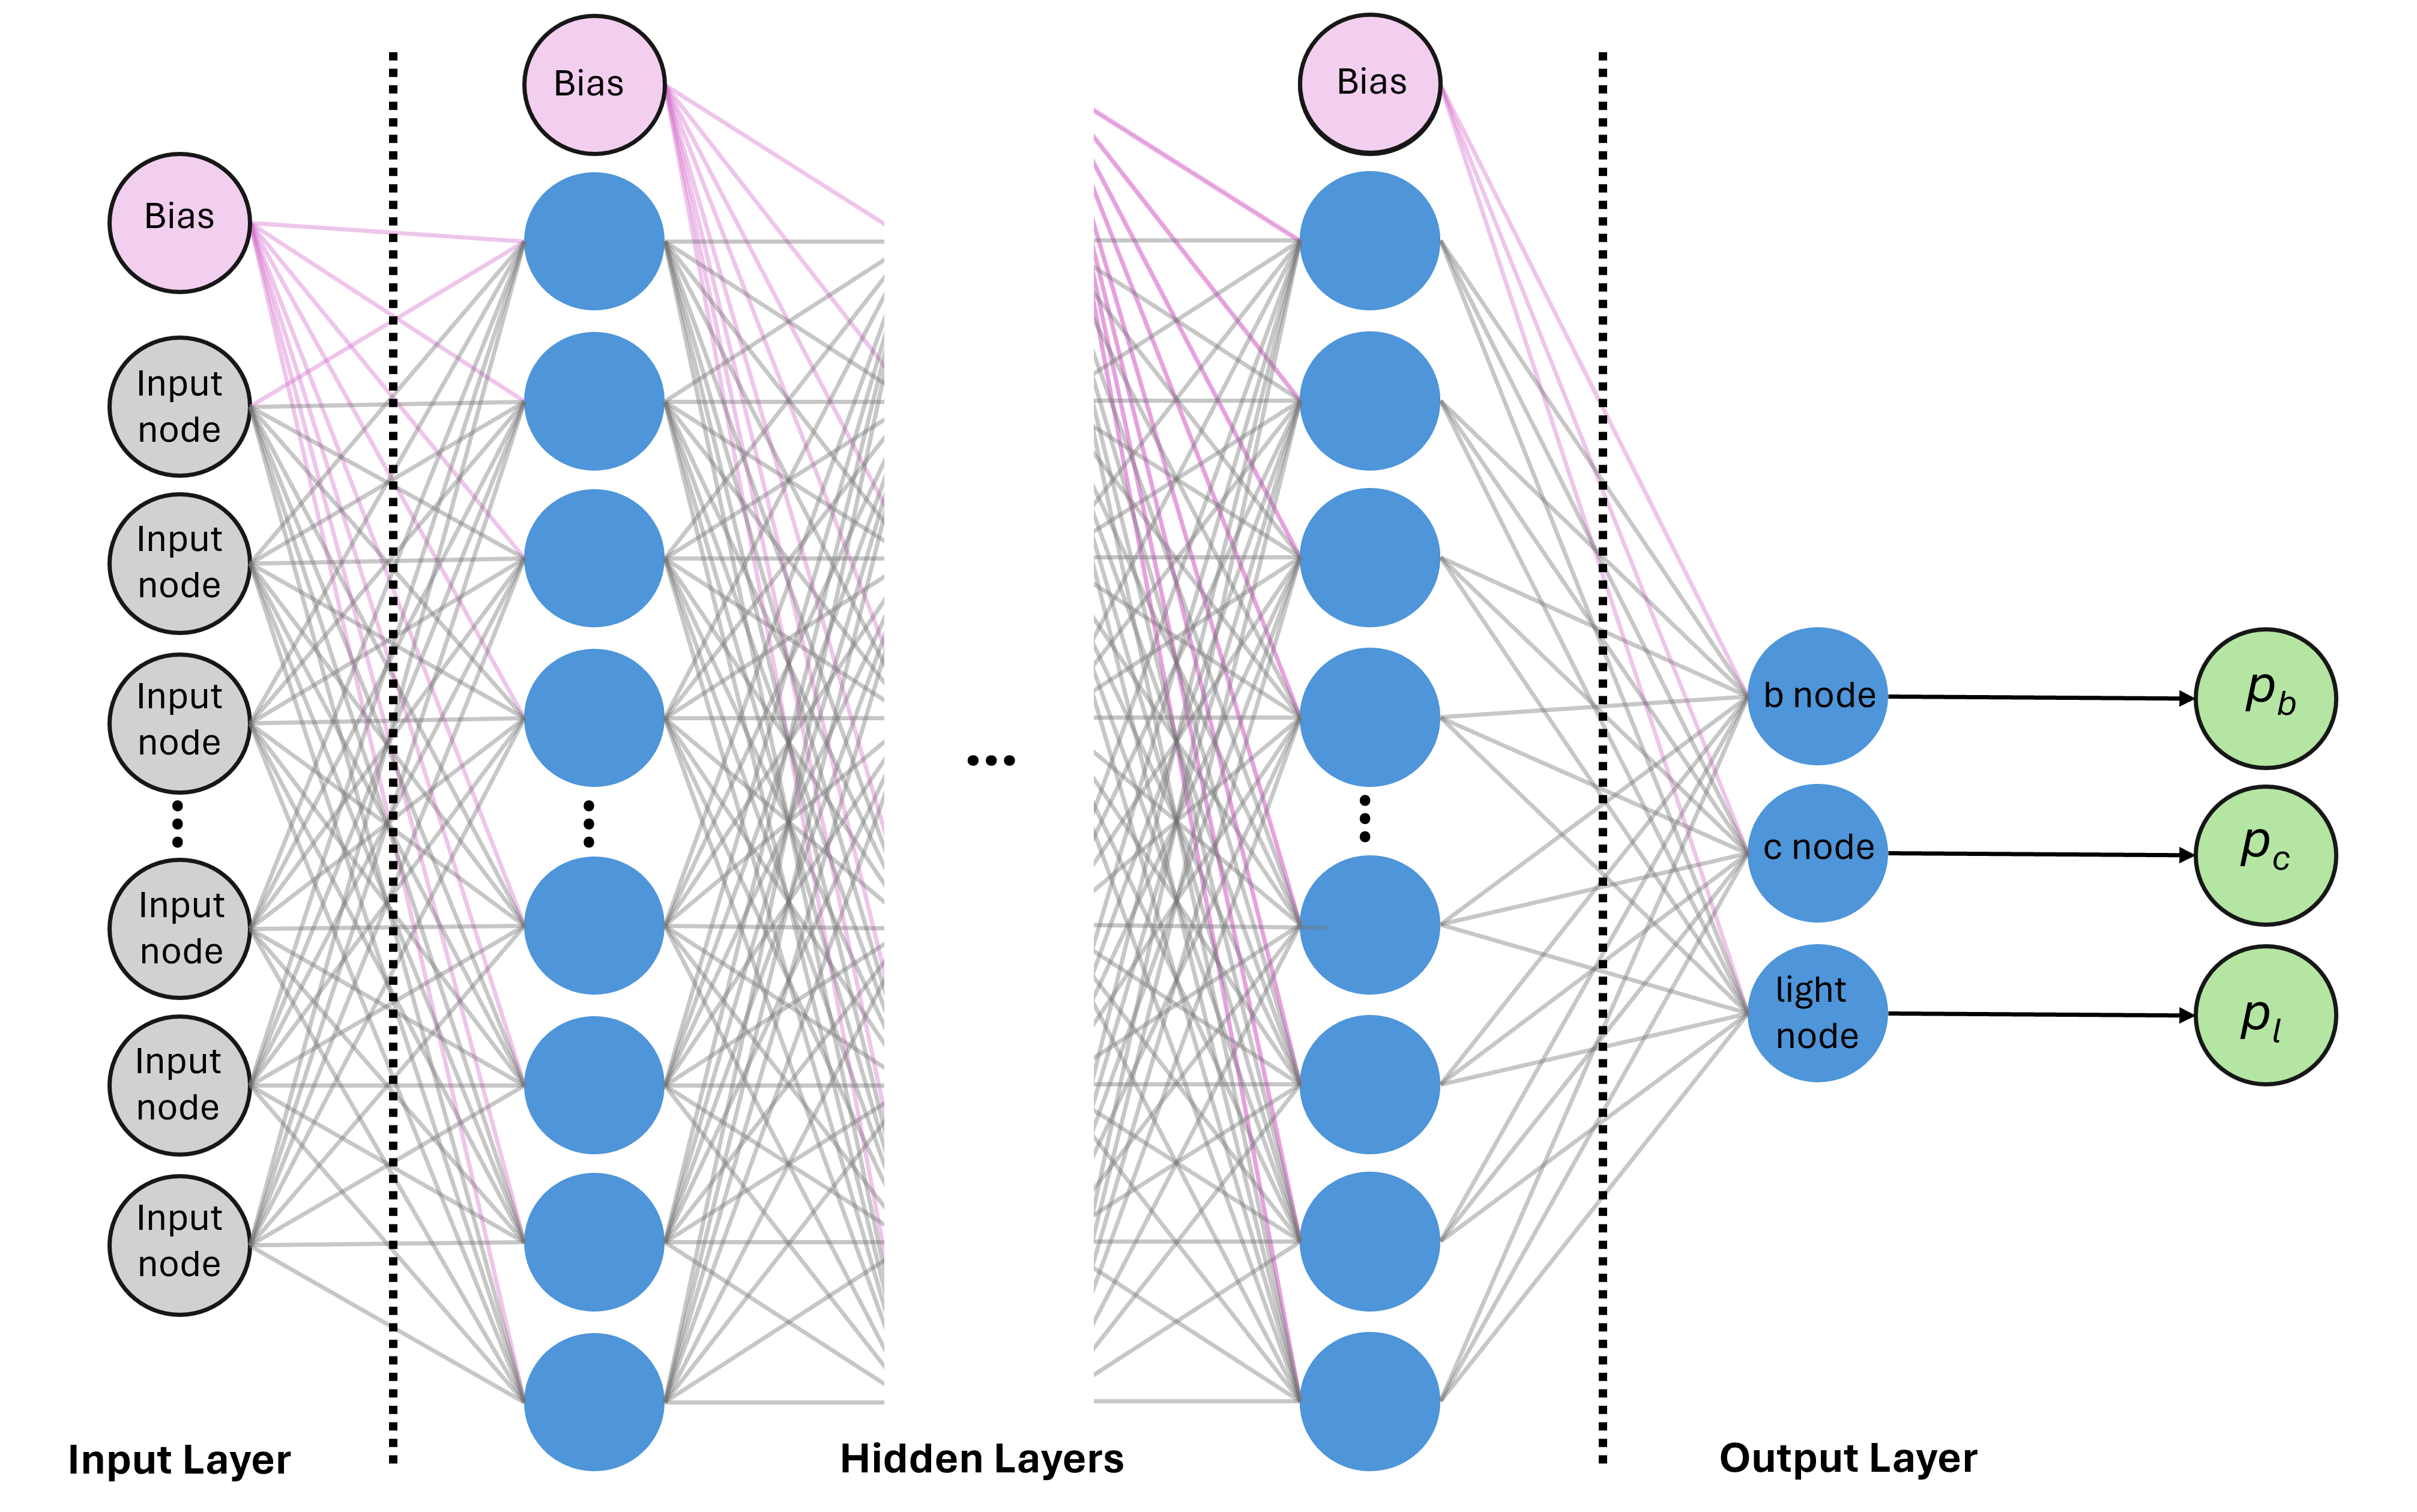
\includegraphics[scale=0.5]{figs/ch5/DL1-arch.png}
    \caption{ Deep feed-forward architecture of DL1 with unspecified number of nodes}
\label{fig:dl1-arch}
\end{figure}
%
As discussed previously, the \gls{dl1} family contains four different types of taggers that utilize different baseline information. The first is the baseline \textit{DL1} that 
uses the same input baseline tagger variables as MV2 (as seen in \ref{tab:ipxd-variables}, \ref{tab:sv1},\ref{tab:jf-btag}) with the additional JetFitter variables for c-tagging 
as seen in table \ref{tab:jf-ctag}. From there the baseline \textit{DL1} is used with additional \gls{nn} inputs. \textit{DL1r} uses the baseline \textit{DL1} with additional 
flavor probabilities from the \gls{rnnip} algorithm. \textit{DL1rmu} exploits the soft-muon information from the muon spectrometer while also including the inputs from the 
\textit{DL1r}. Lastly, the latest tagger is the \textit{DL1d} which is the baseline \textit{dl1} that includes an additional feed-forward \gls{nn} called \gls{dips} that was 
previously discussed in Section \ref{sec:dips}. A diagram of the \gls{dl1} family is seen in Figure \ref{fig:dl1-fam}.

\begin{figure}[h]
    \centering
    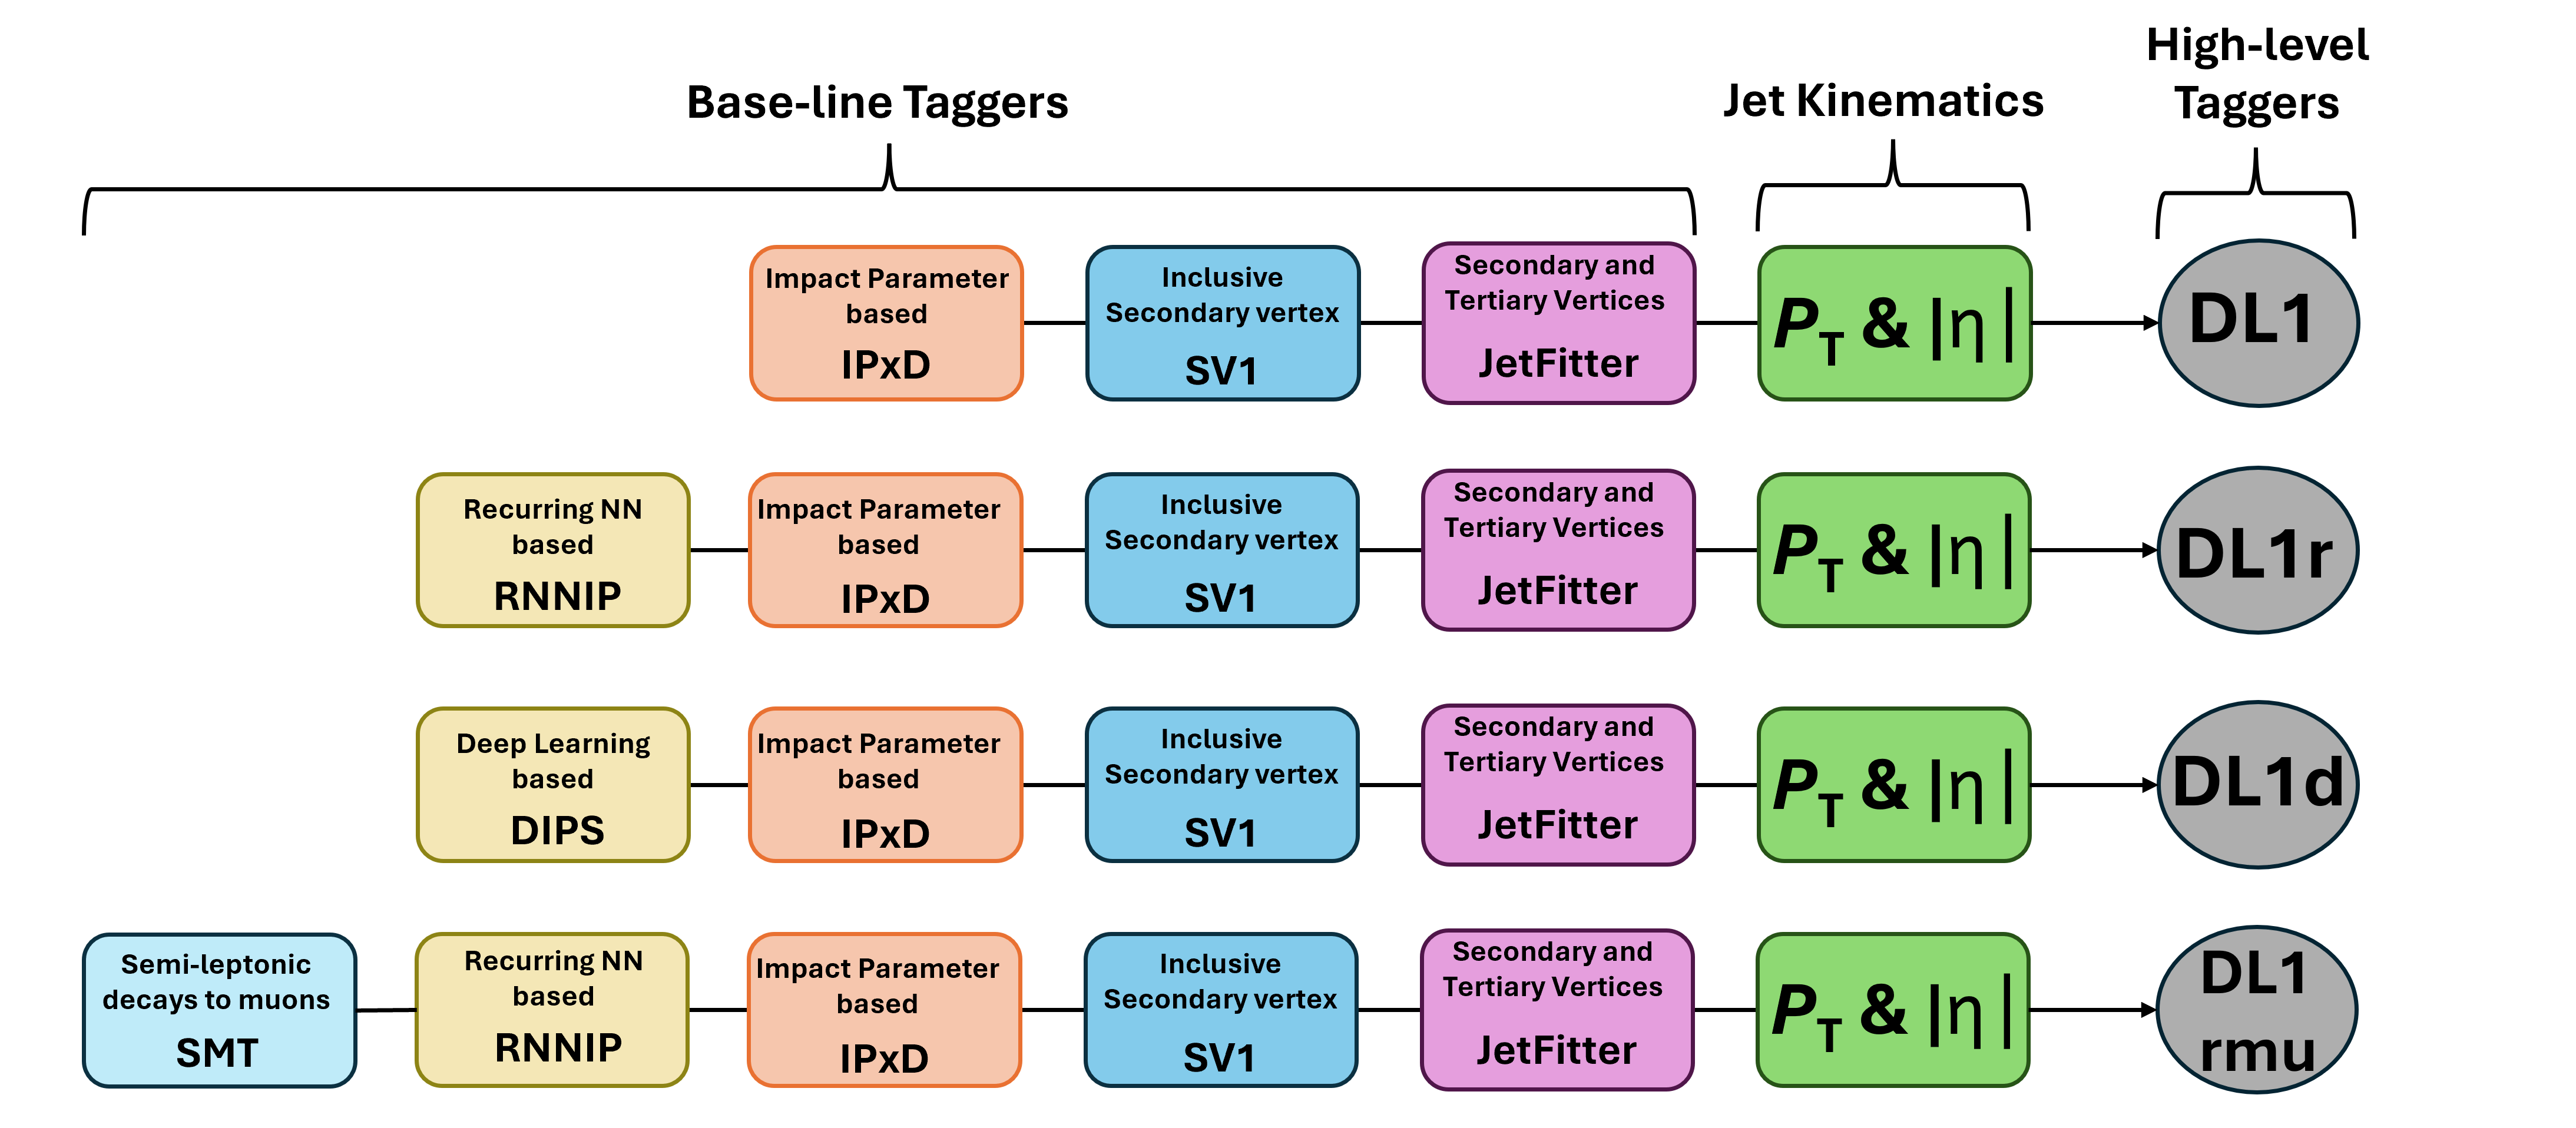
\includegraphics[scale=0.5]{figs/ch5/dl1_fam.png}
    \caption{ Structures of the DL1 tagger family, differing in NN input variables }
\label{fig:dl1-fam}
\end{figure}

\subsection{DL1d design}

In the following sections, training of the DL1d model for the \gls{hllhc} is described. Since the DL1d utilizes the deep learning model \gls{dips}, its design if fairly more complex than the 
other DL1 models in the family. The architecture design can be seen in Figure \ref{fig:dl1d-design}. Notice there are two sub-networks $\upphi$ and \texttt{F} which correspond to the \gls{dips} architecture. The 
\gls{dips} model is trained using track variables described in Table \ref{tab:dips-variables}. Each track in a jet is first processed through the network $\upphi$. In the next step, all \texttt{n}
track networks, corresponding to the number of tracks in a jet, are summed up and further processed via the network \texttt{F}. This can be summarized via an equation as seen:
%
\begin{equation}\label{eq:5.3}
    \overrightarrow{\textrm{P}}_{\textrm{i}} = \texttt{F}\left(\sum_{i=1}^{n}\upphi({\overrightarrow{x}_{\textrm{i}}^{\textrm{t}}})\right)
\tag{5.3}
\end{equation}
%
where $\overrightarrow{x}_{\textrm{i}}^{\textrm{t}}$ are the track input features and $\overrightarrow{\textrm{P}_{\textrm{i}}}$ is the vector of the b-, c-, and light flavor jet class probabilities
corresponding to the \gls{dips} output.

\begin{figure}[h]
    \centering
    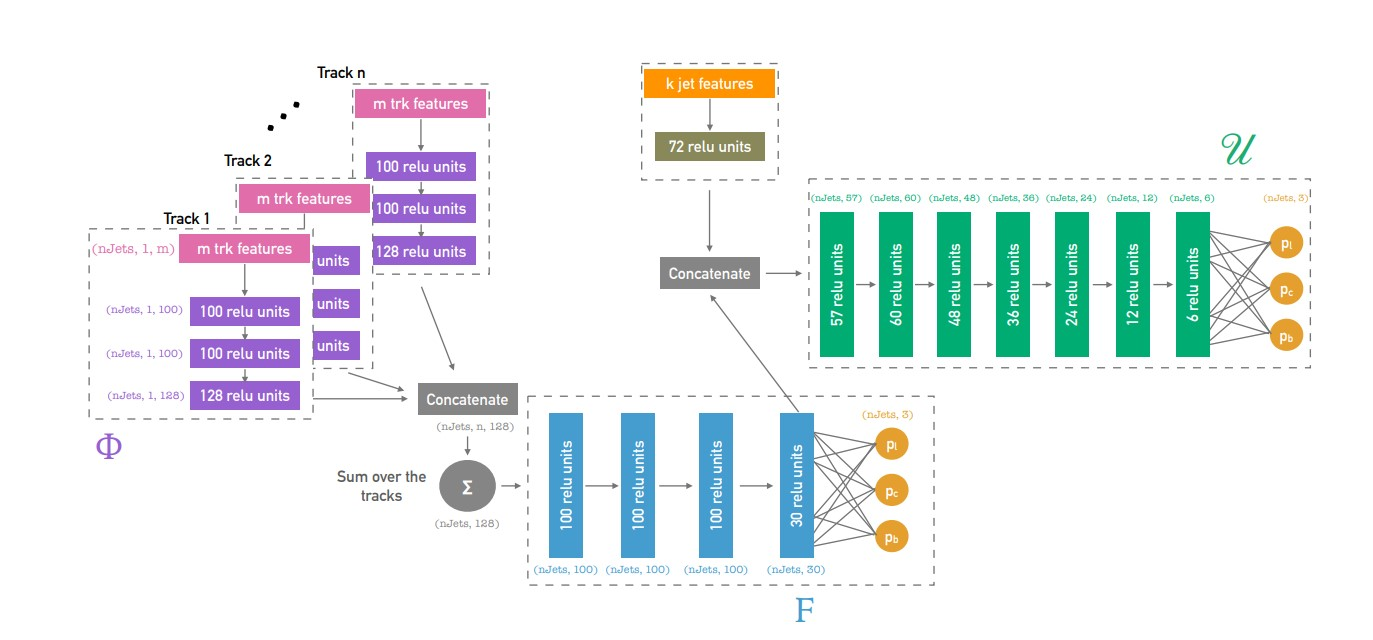
\includegraphics[scale=0.5]{figs/ch5/dl1d-design.jpg}
    \caption{ Architecture of DL1d combining the DIPS $\upphi$ and \texttt{F} networks to the DL1 feed-forward nodes \textit{$\mathscr{U}$} }
\label{fig:dl1d-design}
\end{figure}

The \gls{dips} networks,$\upphi$ and \texttt{F}, are joined to the DL1d feed-forward architecture denoted as \textit{$\mathscr{U}$}. A joint architecture allows the passing of more information into the \gls{dl1} 
\gls{nn} \textit{$\mathscr{U}$}. In the case of Figure \ref{fig:dl1d-arch}, a layer of 30 nodes is concatenated with the other jet features that are processed through a network containing 72 nodes. 
A full back-propagation up to all the track \gls{nn}s $\upphi$ is done during the training allowing a joint optimization of all three networks. The \gls{dips} networks have intermediate losses 
which are used to determine the performance and optimization of the \gls{dips} model prior to being used as input to the \gls{dl1} network. The final feed-forward \gls{dl1} architecture \textit{$\mathscr{U}$}
has three output nodes to calculate the multi-class probabilities. Both networks have dedicated losses. While the loss of the final \textit{$\mathscr{U}$} network \textit{L}($\mathscr{U}$) is sensitive 
to track features and jet kinematics, the loss of \textit{F} network \textit{L}(\textit{F}) is only sensitive to tracks. The overall optimization is performed over the combined loss, as shown:

\begin{equation}\label{eq:5.4}
    \textrm{\textit{L}}(\textrm{comb.}) = \textrm{\textit{L}}(\textit{$\mathscr{U}$}) + \lambda \cdot \textrm{\textit{L}}(\textrm{\textit{F}})
\tag{5.4}
\end{equation}


\section{Software Chain}

The software chain from training the \gls{dl1} tagger to validation and deployment in the \gls{atlas} software \texttt{ATHENA} are unassociated. The training of the \gls{nn} 
is based on the industry-standard open-sourced coding language Python3.6~\cite{python}. The packages numpy~\cite{numpy} and pandas~\cite{pandas} are used for data handling
while it's formatted in the HDF5 format~\cite{hdf5}. The \gls{atlas} software package developed to convert root datasets into HDF5 format is called the Training Dataset Dumper (\gls{tdd})
The code structure is configured using human-readable formats such as JSON~\cite{json} and yaml to ensure user compatibility.
For the \gls{nn} training, Tensorflow~\cite{tensorflow} is used with a Keras2~\cite{keras} frontend. These packages are used to create a user-friendly framework for deep learning training 
called Umami which handles the preprocessing and training steps. For visualization, the package matplotlib~\cite{matplotlib}  and tools from 
scikit-learn~\cite{scikit} are included in the training scripts. These tools are compiled into a convenient tool in the Umami family named Puma. The full workflow (Umami and Puma) can be 
performed using a Docker image~\cite{docker} which allows the software to be ran 
from any computer without the need to install the necessary environment. The output model is then transformed into a format called LightWeight Tagger Neural Network~\cite{lwtnn} (\gls{lwtnn})
which integrates the model into the \gls{atlas} software \texttt{ATHENA}.

\section{Preprocessing}

The first step before training a \gls{dl1} model is preparing the input in a step called \textit{preprocessing}. To ensure robustness of a model to perform properly over a large 
$\textrm{\textit{p}}_{\textrm{T}}$ spectrum, two simulated samples are combined into a \textit{hybrid sample}. One sample is of $t\bar{t}$ events and the other is of a \gls{bsm} particle 
called $\textrm{Z}'$. An example $\textrm{\textit{p}}_{\textrm{T}}$ spectrum of these two samples can be seen in Figure \ref{fig:hybrid-noscale} in (a). The $\textrm{Z}'$ allows a flat $\textrm{\textit{p}}_{\textrm{T}}$ spectrum of up to 4.5 TeV with a 
total range up to 6 TeV. This $\textrm{Z}'$ sample is known as an \textit{extended $\textrm{Z}'$} sample since the normal distribution of a $\textrm{Z}'$ is up to about $\approx$4 TeV. The $t\bar{t}$ sample populates the lower $\textrm{\textit{p}}_{\textrm{T}}$ spectrum, ensuring there are enough statistics for a proper model to be trained while the $\textrm{Z}'$ populates 
larger $\textrm{\textit{p}}_{\textrm{T}}$ to increase tagging efficiencies for heavier particles. This sample, along with all that is included in this thesis, are using PFlow objects. 
The object selection within the $t\bar{t}$ sample is of the following:
%
\[
 t\bar{t} \ \textrm{selection :} \begin{cases}
       \textrm{b-jets} & \textrm{b-hadron} \ \textrm{\textit{}}_{\textrm{T}} < \textrm{250 GeV}\\ 
       \textrm{c-jets} & \textrm{jet} \ \textrm{\textit{p}}_{\textrm{T}} < \textrm{250 GeV}\\
       \textrm{light-jets} & \textrm{jet} \ \textrm{\textit{p}}_{\textrm{T}} < \textrm{250 GeV}\\
\end{cases}\]
%
As noted here, the b-jet selection uses b-hadron $\textrm{\textit{p}}_{\textrm{T}}$. The sample fraction of $t\bar{t}$ and $\textrm{Z}'$ can be adjusted, in the following example plots, 
the fraction is adjusted to 70\% $t\bar{t}$ and 30\% $\textrm{Z}'$. The merged \textit{hybrid sample} can be seen in (b) of Figure \ref{fig:hybrid-noscale}.

\begin{figure}[h]
    \centering
    \subfloat[\centering ]{{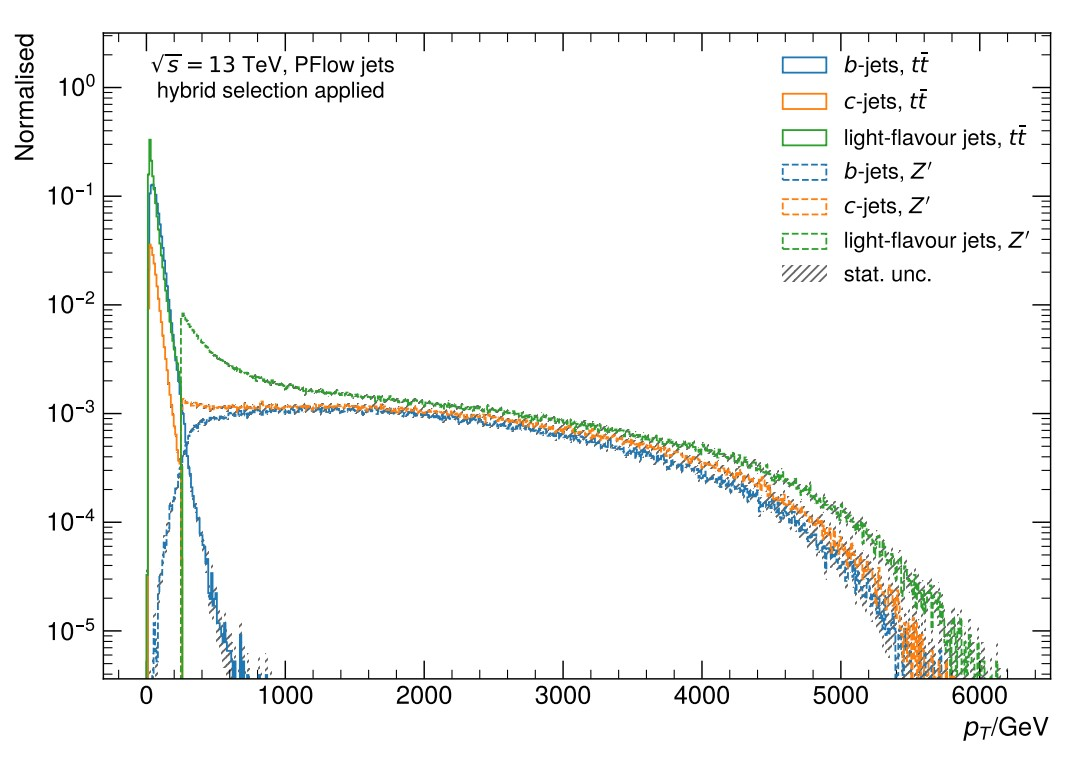
\includegraphics[scale=0.29]{figs/ch5/nohybrid_noscale.jpg}}}%
    \subfloat[\centering ]{{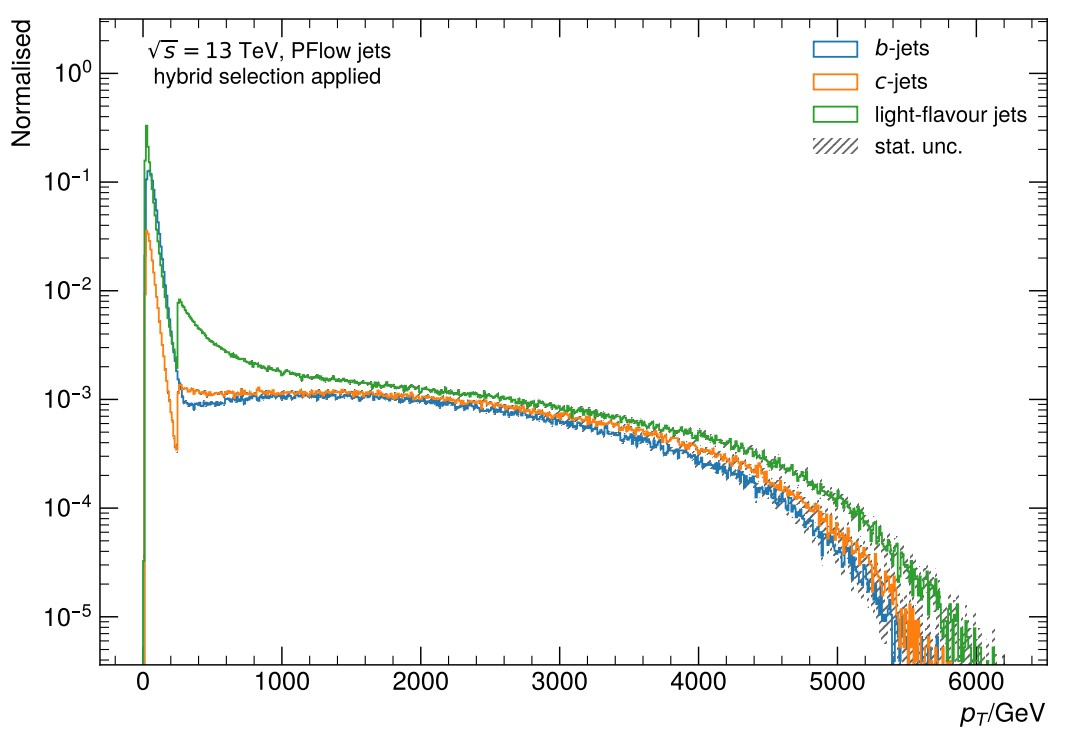
\includegraphics[scale=0.29]{figs/ch5/hybrid_noscale.jpg}}}%
    \caption{  (a) $\textrm{\textit{p}}_{\textrm{T}}$ distribution of $t\bar{t}$ sample (solid lines) and a Z$'$ sample (dashed lines). The $t\bar{t}$ b-jet distribution is normalized to unity and all other distributions are normalized to the b-jet distribution. (b) Samples from (a) merged into one distribution normalized to b-jet distribution }
\label{fig:hybrid-noscale}
\end{figure}

The goal of the \gls{dl1} tagger is to differentiate between hadron flavors. As seen in Figure \ref{fig:sample_fractions}, the flavor composition is imbalanced towards light-flavor 
jets. In order to avoid kinematic and count biases within the tagger, a resampling step must be applied. This also helps mitigate discontinuity between the two 
combined samples. Kinematic correlations are important for the baseline taggers, the goal for the high-level tagger is to avoid differences in kinematics and attempt to tag hadrons 
by jet-by-jet classification. Instead of weighting each sample fraction to match a chosen distribution, a resampling method is deployed to avoid instabilities in the model training 
steps. There are two methods of resampling. There is \textit{undersampling} where single jets are removed from the majority classes to fit a distribution of a minority class or 
there is \textit{oversampling} where jets from minority classes are duplicated to match a given distribution. Figure \ref{fig:resampling_diagram} shows a diagram of both methods. A combined method called 
Importance Sampling with Replacement, also referred to as \textit{PDF} sampling, undersamples and oversamples distributions to match a middle target distribution while enforcing the 
same shape. As seen in Figure \ref{fig:sample_fractions}, b-jets are a middle distribution, therefore the PDF sampling is used in the preprocessing step of the following work.

\begin{figure}[h]
    \centering
    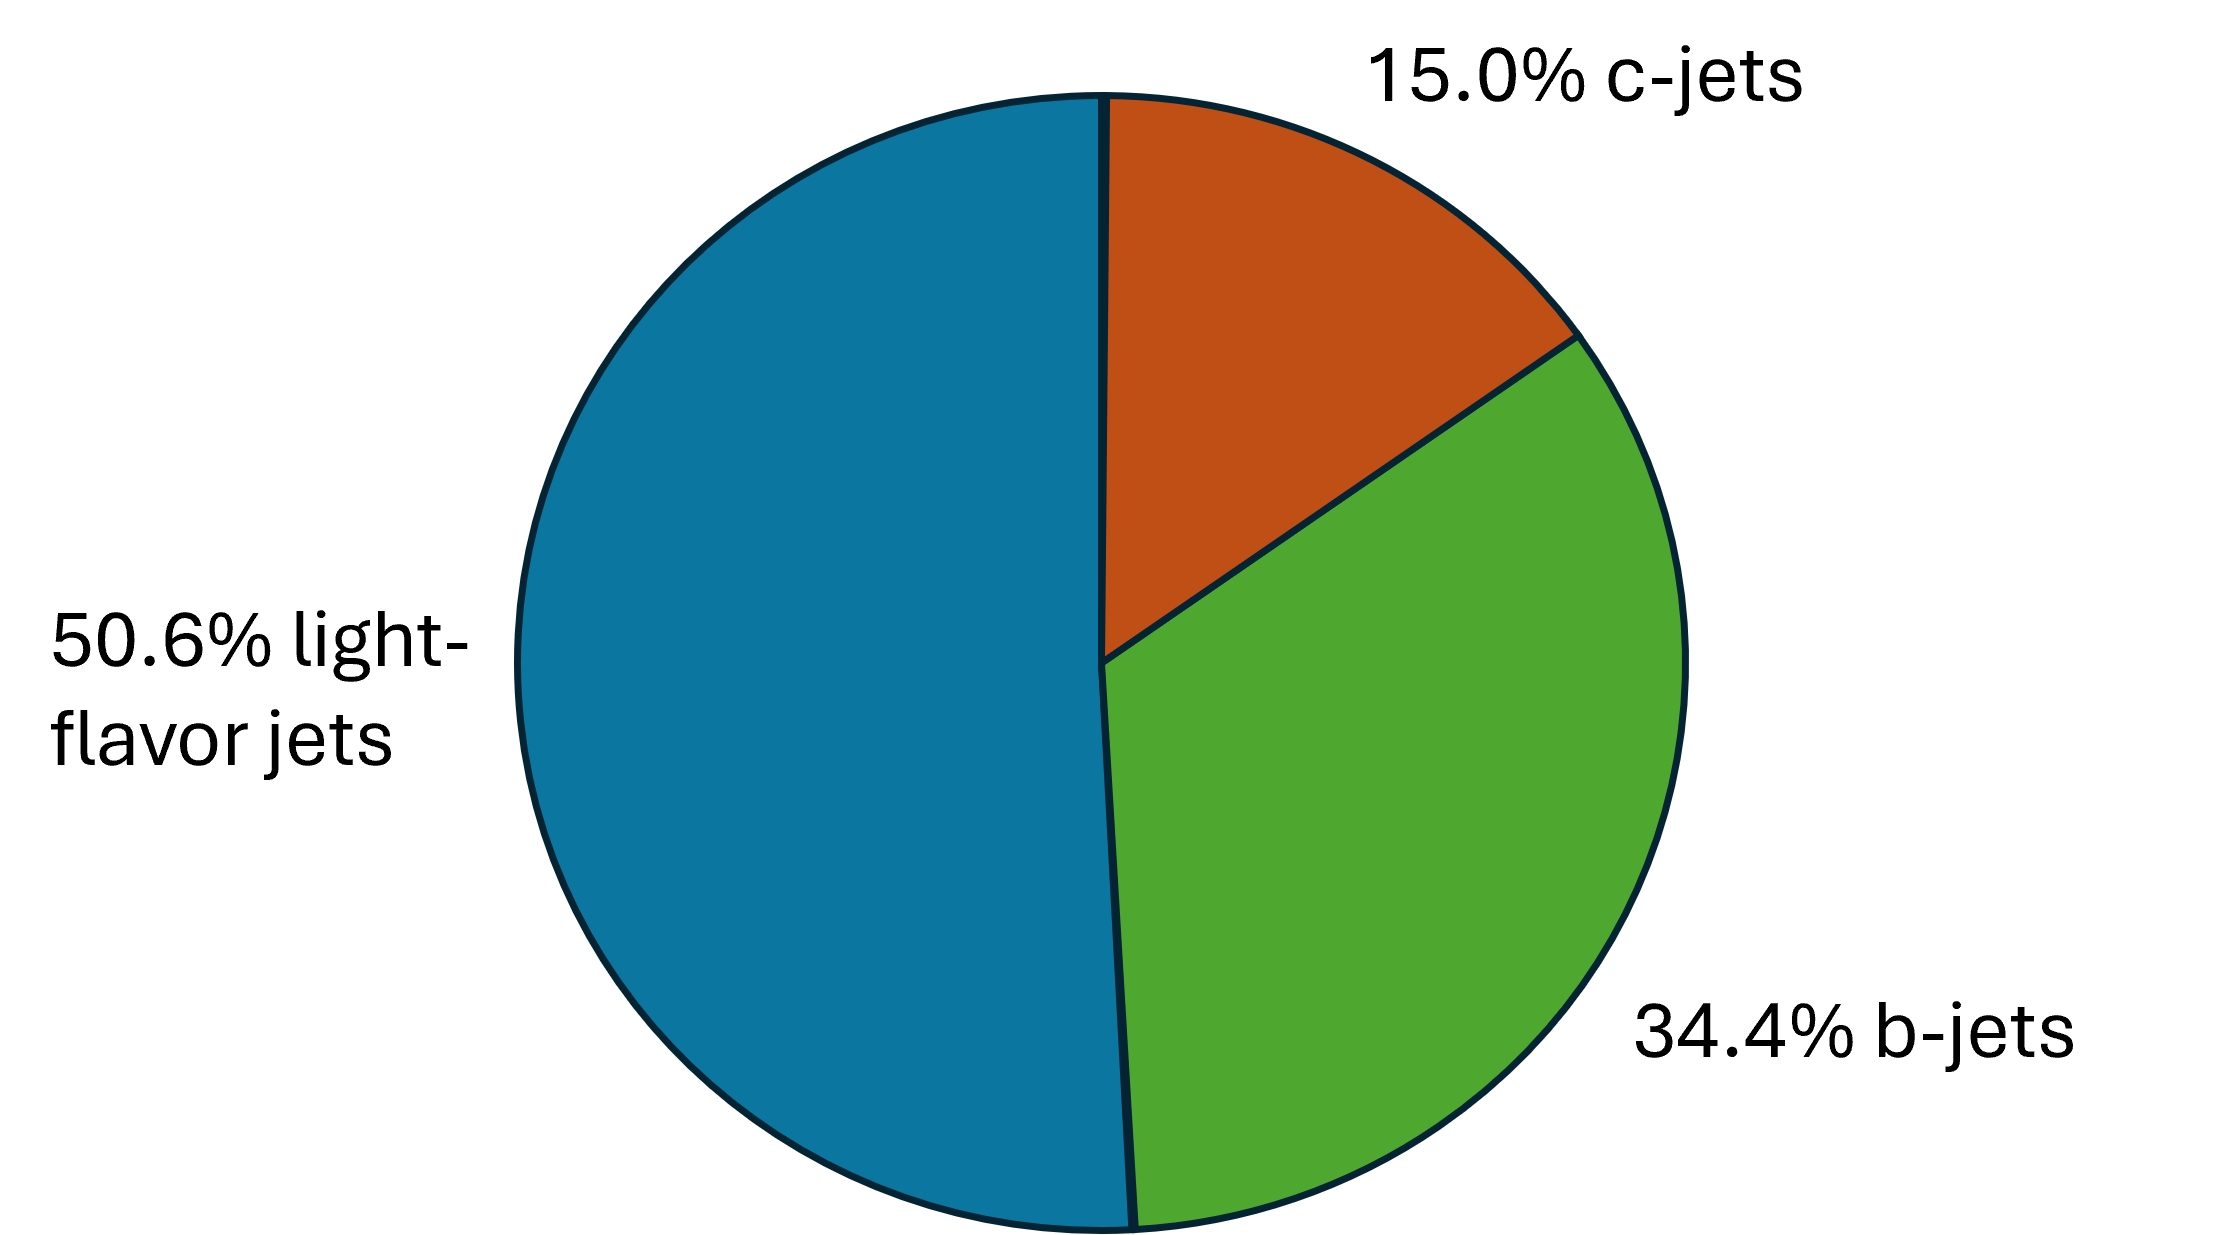
\includegraphics[scale=0.6]{figs/ch5/ex_comp_pie.png}
    \caption{ Hybrid sample hadron fractions.}
\label{fig:sample_fractions}
\end{figure}

\begin{figure}[h]
    \centering
    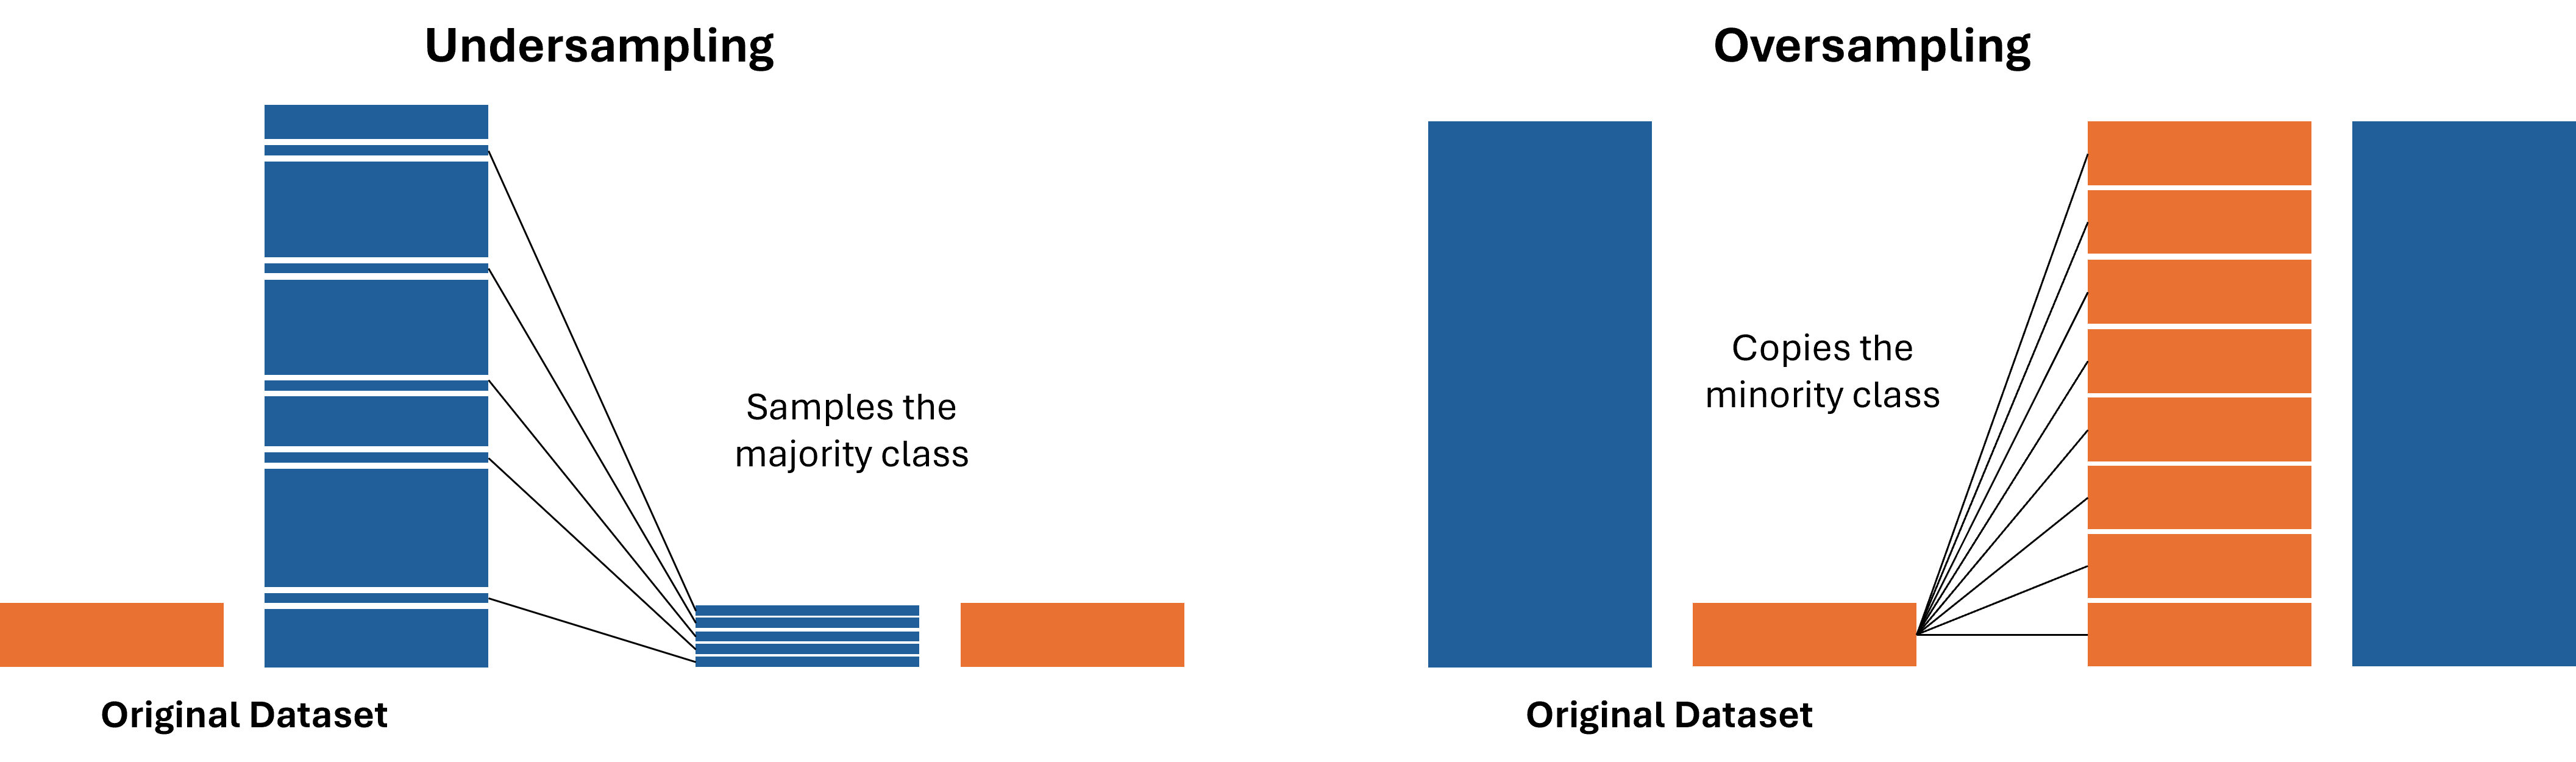
\includegraphics[scale=0.5]{figs/ch5/Sampling-diagram.png}
    \caption{ Diagram of the resampling methods to ensure balanced model training.}
\label{fig:resampling_diagram}
\end{figure}

The obvious issue that is present in these sampling methods is the duplication of events during oversampling a minority distribution. This may cause 
a bias due to the lack of diversity of statistics in the minority groups. Luckily, the samples are \gls{mc} produced and therefore the statistics can be
simply increased by producing more samples through event generators. However, a resampling procedure referred to as the \textit{count method} was studied as a comparison
to the PDF method. The count method strictly only undersamples to the lowest distribution, thus drastically decreasing statistics in favor of bias possibilities. 
The $\textrm{\textit{p}}_{\textrm{T}}$ and $|\textrm{η}|$ b-jet distributions are taken as 
reference and the c-jet and light-jet flavor are resampled to match them. The binning used for the undersampling procedure tends to be more granular, especially 
in the lower $\textrm{\textit{p}}_{\textrm{T}}$ region where the sample transition bins are, while at higher $\textrm{\textit{p}}_{\textrm{T}}$ the bins are wider. This can 
be seen by resampling the example distribution from Figure \ref{fig:hybrid-noscale} in Figure \ref{fig:hybrid-scaled}.

\begin{figure}[h]
    \centering
    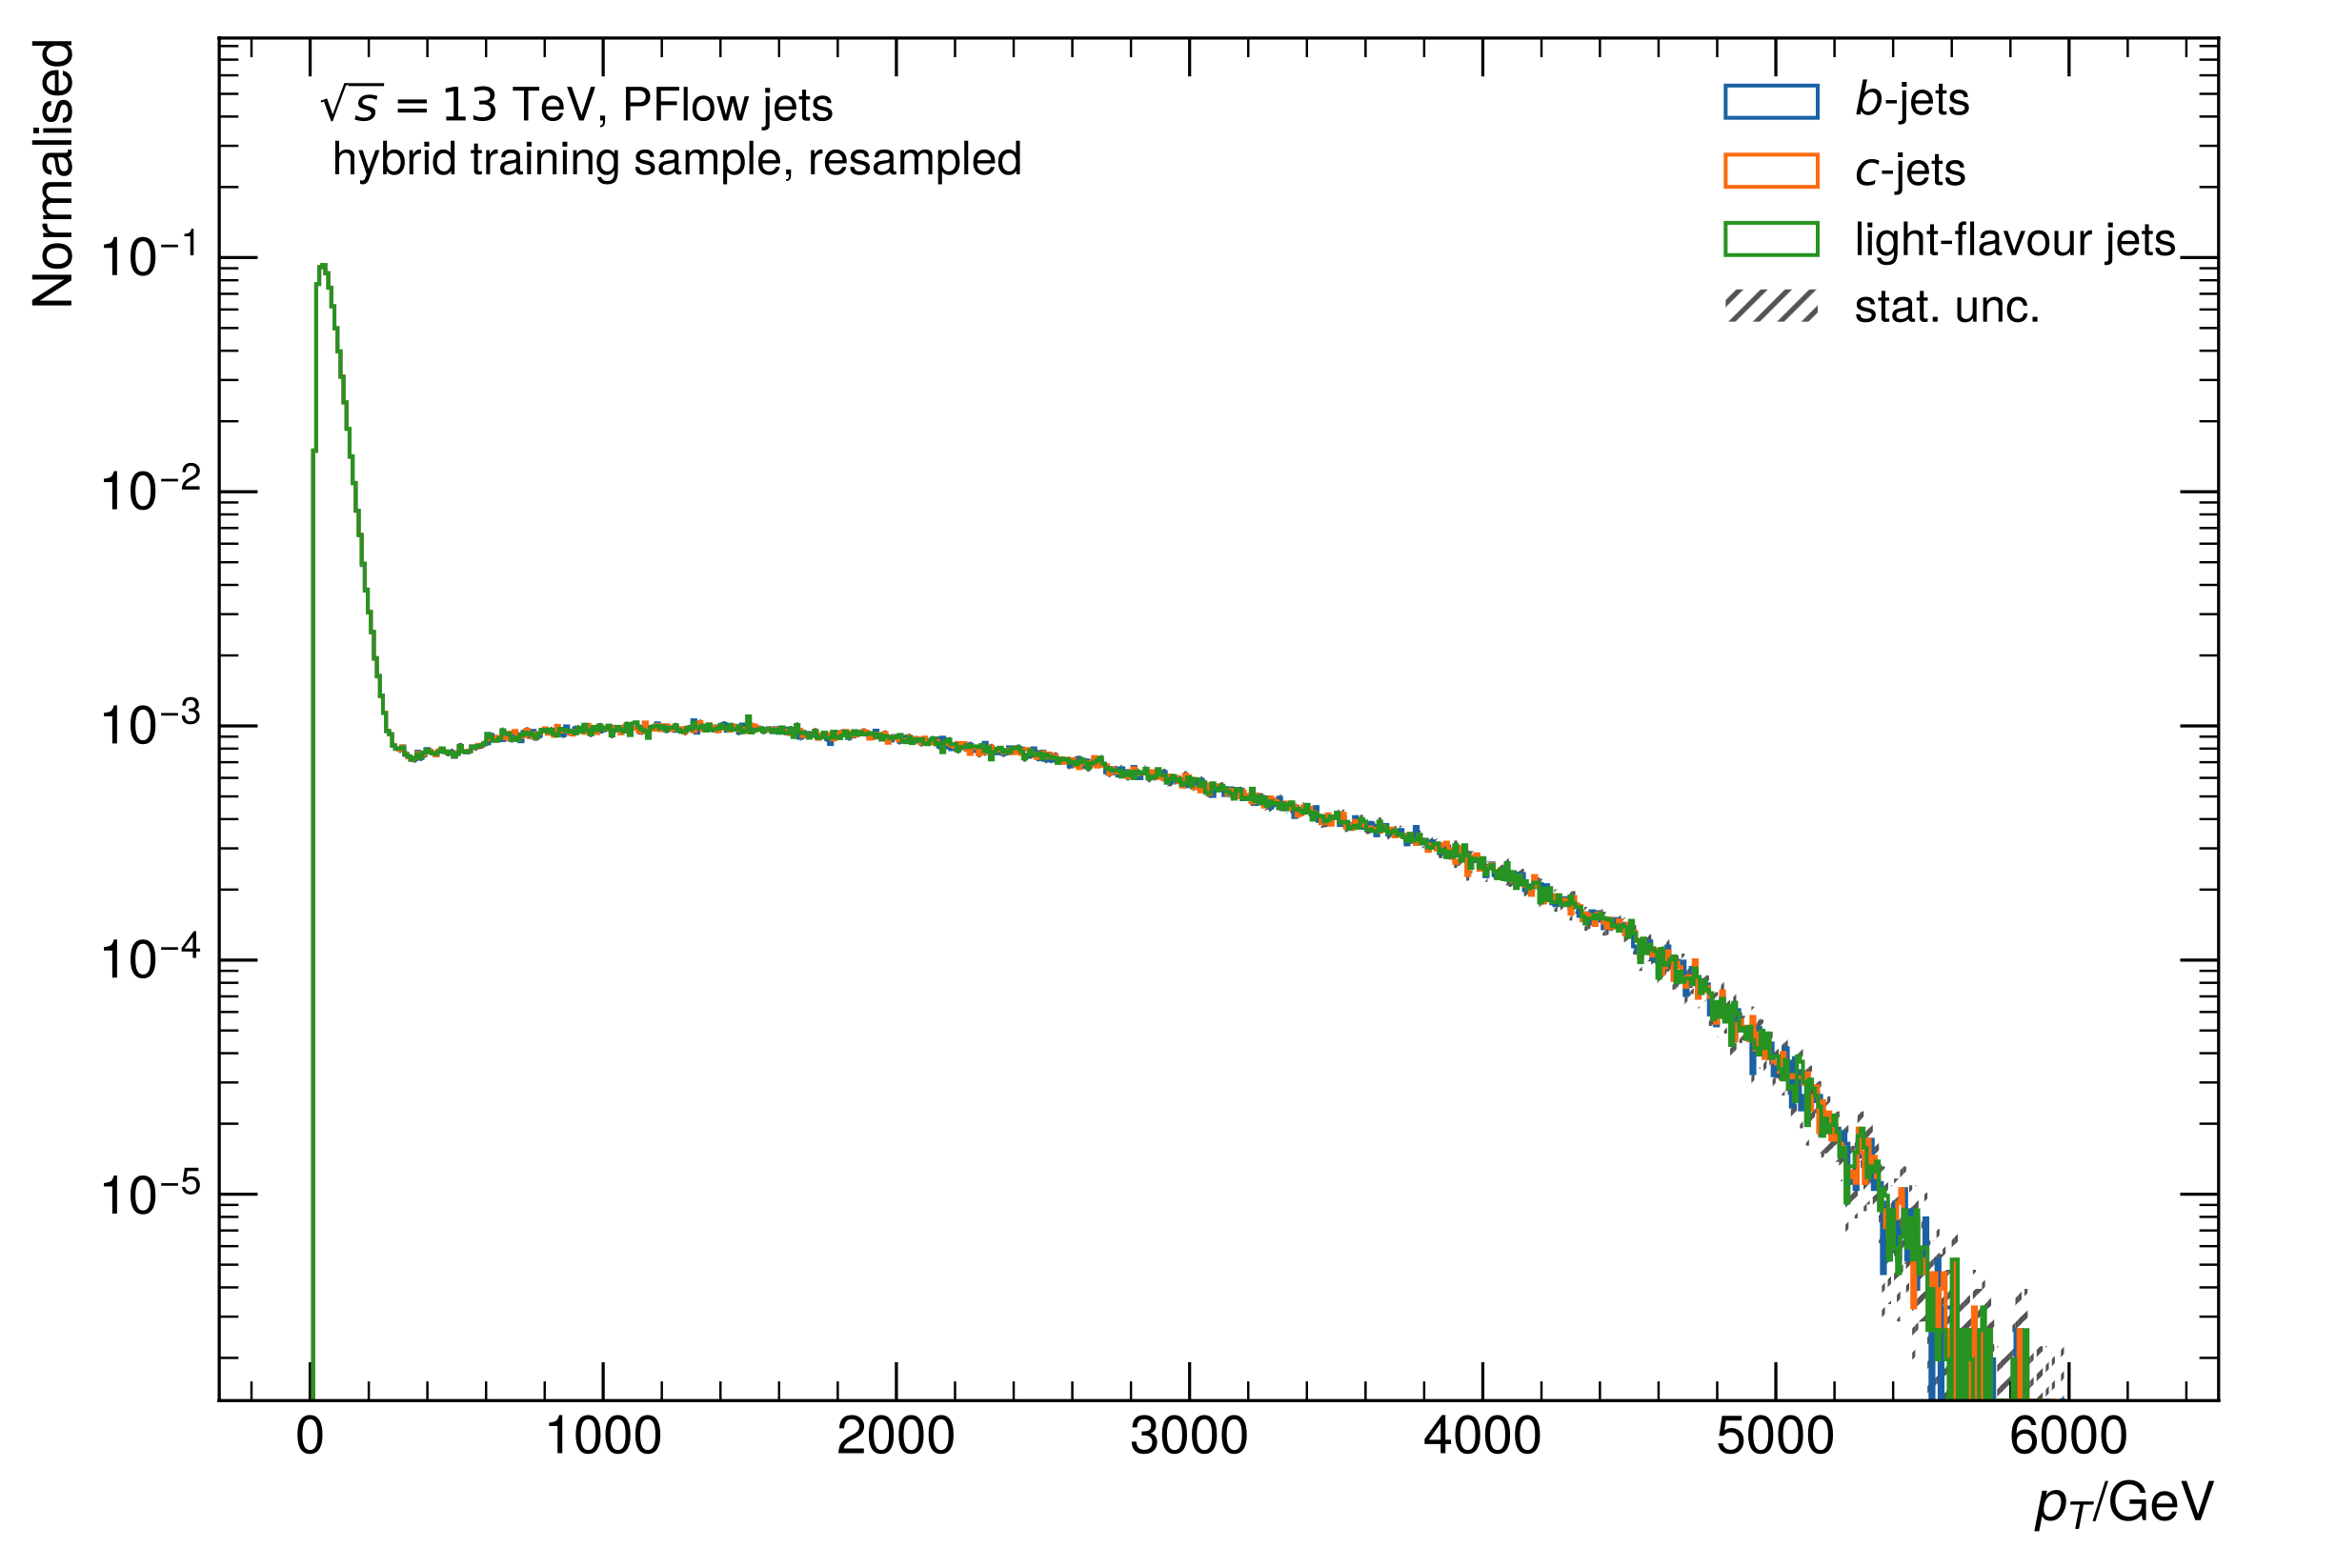
\includegraphics[scale=0.35]{figs/ch5/hybrid-scaled.png}
    \caption{ Resampled example flavor distributions.}
\label{fig:hybrid-scaled}
\end{figure}

Lastly before training, the ranges of the input variables need to be balanced so that they're all in the same order of magnitude, otherwise certain 
variables would carry more weight in the model training procedure. Therefore, all the variables are shifted to a mean of zero and a standard deviation 
of one, with the exception of binary check variables. Also, extremely anomalous events originating from obscure phase spaces within the samples are 
removed to secure an undisturbed training process.

\section{ HL-LHC Samples}

The current versions of these heavy-flavor taggers have been trained using simulated samples from Run 2. The latest versions that are being implemented as of 2023 have been 
optimized for Run 3 and are trained on the latest Run 3 samples. In the scope of this thesis, preliminary trainings for the DL1 tagger have been conducted using samples 
simulated using the \gls{itk} from Run 4 that starts in 2029 in order to see how well the new geometry can increase tagging efficiency with the main focus on the increase 
of $|\textrm{η}| \le$ 4. All objects simulated in these samples are PFlow objects as discussed in Section \ref{sec:small-R}.

\subsection{Object Selections}

The most important features for training effective taggers are tracks, therefore it's vital to simulate tracks through the new \gls{itk} detector with precision. These tracks represent 
trajectories of charged particles reconstructed from hits in the \gls{itk} pixels and strip sensors. The η-dependent variables underwent a combination of selections based on general track quality criteria and requirements 
specific to flavor tagging algorithms. The variables used in the baseline taggers (found in tables \ref{tab:ipxd-variables}, \ref{tab:sv1}, \ref{tab:jf-btag}) have adjusted criteria due to the 
pseudorapidity extension of the \gls{itk} detector. Only jets with $\textrm{\textit{p}}_{\textrm{T}} >$ 20 GeV and $|\textrm{η}| \le$ 4 are considered. A generator-level overlap removal with electrons 
and muons from W boson decays are also applied. Pile-up jet rejection algorithms are still under development for the \gls{hllhc}, so the selected jets are required to be matched within $∆\textrm{R} >$
0.3 with truth-jets built from hard-scatter stable particles that are clustered with the anti-$\textrm{\textit{k}}_{\textrm{T}}$ algorithm with R=0.4. The selected reconstructed primary vertex is required to be within 1 mm 
of the hard scatter vertex. Tracks are associated to jets using $\textrm{\textit{p}}_{\textrm{T}}$-dependent matching criteria, with a cone size of $∆\textrm{R} \approx$ 0.45 for jets with $\textrm{\textit{p}}_{\textrm{T}}$
= 20 GeV to $∆\textrm{R} \approx$ 0.25 for jets with $\textrm{\textit{p}}_{\textrm{T}} >$ 200 Gev. In cases where multiple tracks pass the criteria, the closest track is chosen. Jet flavor labels are assigned 
based on generator-level presence of b- or c-hadrons, or $\tau$ hadronic decays. If a b-hadron with $\textrm{\textit{p}}_{\textrm{T}} >$ 5 GeV is found within $∆\textrm{R}$ = 0.3, the jet is labeled a b-jet. 
This procedure is repeated for c-hadrons and $\tau$ hadronic decay products. Jets that have no labels by the end of this iteration are assumed to originate from light-flavor quarks and 
are labeled light-jets. Table \ref{tab:itk-req} shows the new requirements imposed on the jets due to the implementation of the \gls{itk} detector.

\begin{table}[ht]
    \centering 
    \begin{tabular}{ |c | c | c| c |}
        \hline
        \multicolumn{4}{|c |}{New Flavor Tagging Requirements for ITk}\\
        \hline\hline
        Requirements & \multicolumn{3}{|c|}{Pseudorapidity interval} \\ \cline{2-4}
                     & $|\textrm{η}|<$ 2 & 2.0 $< |\textrm{η}|<$ 2.6 & 2.6 $<|\textrm{η}|<$ 4.0 \\ 
        \hline
        pixel + strip hits & $\geq$ 9 &  $\geq$ 8 & $\geq$ 7 \\
        pixel hits & $\geq$ 1 & $\geq$ 1 & $\geq$ 1 \\
        pixel + strip holes & $\leq$ 2 & $\leq$ 2 & $\leq$ 2 \\
        $\textrm{\textit{p}}_{\textrm{T}}$ [MeV] & $>$ 900 & $>$ 500 & $>$ 500 \\
        $|\textit{\textrm{d}}_{\textrm{0}}|$ [mm] & $\leq$ 2.0 & $\leq$ 2.0 & $\leq$ 3.5 \\
        $|\textit{\textrm{z}}_{\textrm{0}}\textrm{sin}\theta|$ [mm] & $\leq$ 5.0 & $\leq$ 5.0 & $\leq$ 5.0 \\
        \hline
    \end{tabular}
    \caption{Training samples used for DL1d for HL-LHC studies \cite{run4-ftag}}
    \label{tab:itk-req}
\end{table}


\subsection{Sample Preprocessing}


The following samples consist of the necessary $t\bar{t}$ and $\textrm{Z}'$ samples for training with a \gls{cme} of 14 TeV which aligns with the predicted \gls{hllhc} beam energy. A small
sample of only 100,000 events is also used that include thes \gls{hgtd} (briefly discussed in Section \ref{sec:hgtd}) detector within the simulation step and is used for a few studies that are 
mentioned later in this chapter. These three samples are listed in table \ref{tab:dl1-samples}.


\begin{table}[ht]
    \centering 
    \begin{tabular}{ |c | c | c| c |c |}
        \hline
        \multicolumn{5}{|c |}{HL-LHC DL1 Training Samples}\\
        \hline\hline
        Sample & \multicolumn{0}{c}{Container} & & $\langle \upmu \rangle$ & \# of Events\\
        \hline
        $t\bar{t}$    & \multicolumn{1}{l}{mc15\_14TeV.600012.PhPy8EG\_A14\_ttbar\_hdamp258p75} & & 200 & 4,374,000\\
         & \multicolumn{0}{l}{\_nonallhad.recon.AOD.e8185\_s3654\_s3657\_r12573} & &  &   \\
        $\textrm{Z}'$ & \multicolumn{1}{l}{mc15\_14TeV.800030.Py8EG\_A14NNPDF23LO\_flatpT} & &   200 & 1,605,205 \\
         & \multicolumn{0}{l}{\_Zprime\_Extended.recon.AOD.e8185\_s3654\_s3657\_r12574}  & & & \\
         HGTD & \multicolumn{1}{l}{mc15\_14TeV.600012.PhPy8EG\_A14\_ttbar\_hdamp258p} & &   200 & 100,000 \\
         & \multicolumn{0}{l}{75\_nonallhad.recon.AOD.e8185\_s3770\_s3773\_r13618}  & & & \\
        \hline
    \end{tabular}
    \caption{Training samples used for DL1d for HL-LHC studies}
    \label{tab:dl1-samples}
\end{table}

The values corresponding to the letters in the latter half of the container names correspond to certain production versions. Table \ref{tab:sample-nomen} shows the nomenclature for these values.
\hspace{-3mm}
\begin{table}[H]
    \centering 
    \begin{tabular}{ |c | c | c| c |}
        \hline
        \multicolumn{4}{|c |}{Sample Production Nomenclature}\\
        \hline\hline
        Prod. Step Name & Prod. Step Tag & \multicolumn{0}{c}{Definition} & \\
        \hline
        evgen & e & \multicolumn{0}{l}{Event generation tag. MC generation of quark-gluon } & \\
         & & \multicolumn{0}{l}{interactions to parton showering and hadronization} & \\
        simul & s & \multicolumn{0}{l}{Simulation tag corresponds to simulated detector} & \\
         & & \multicolumn{0}{l}{hits when using MC simulations} &  \\
        digit & d & \multicolumn{0}{l}{Digitization tag is turning the simulated energy} & \\
         & & \multicolumn{0}{l}{deposits into detector response that resembles raw data} & \\
        recon & r & \multicolumn{0}{l}{Reconstruction tag corresponds to the offline reconstruction} & \\
         & &  \multicolumn{0}{l}{algorithm release used to build physics objects} & \\
        deriv & p & \multicolumn{0}{l}{Derivation p-tag refers to a derivation framework used} & \\
         & &  \multicolumn{0}{l}{to obtain useful physics objects} &  \\
        \hline
    \end{tabular}
    \caption{Training samples used for DL1d for HL-LHC studies}
    \label{tab:sample-nomen}
\end{table}

In order to finalize the preparation of these samples, they had to be prepared and resampled due to their imbalance of hadron flavors. The imbalance in both of the upgrade samples are
shown in Figure \ref{fig:comp-pie}. In order to prepare these samples, both of them were combined into a hybrid sample consisting of 70\% $t\bar{t}$ and 30\% $\textrm{Z}'$ events.
Next, the dataset is split into three different sets. The first is the training set, this one is the largest of the three 
in order to maximize training statistics. The other two sets are the validation set used to validate the model and lastly is the testing set which tests the model afterwards. 
The resampling process of PDF, as previously described in the last section, was used to match the b-hadron distribution whereas the count method undersamples to the lowest 
distribution which happens to be c-jets. Table \ref{tab:training-stats} breaks down the sample statistics for each dataset and resampling method. 

\begin{figure}[h]
    \centering
    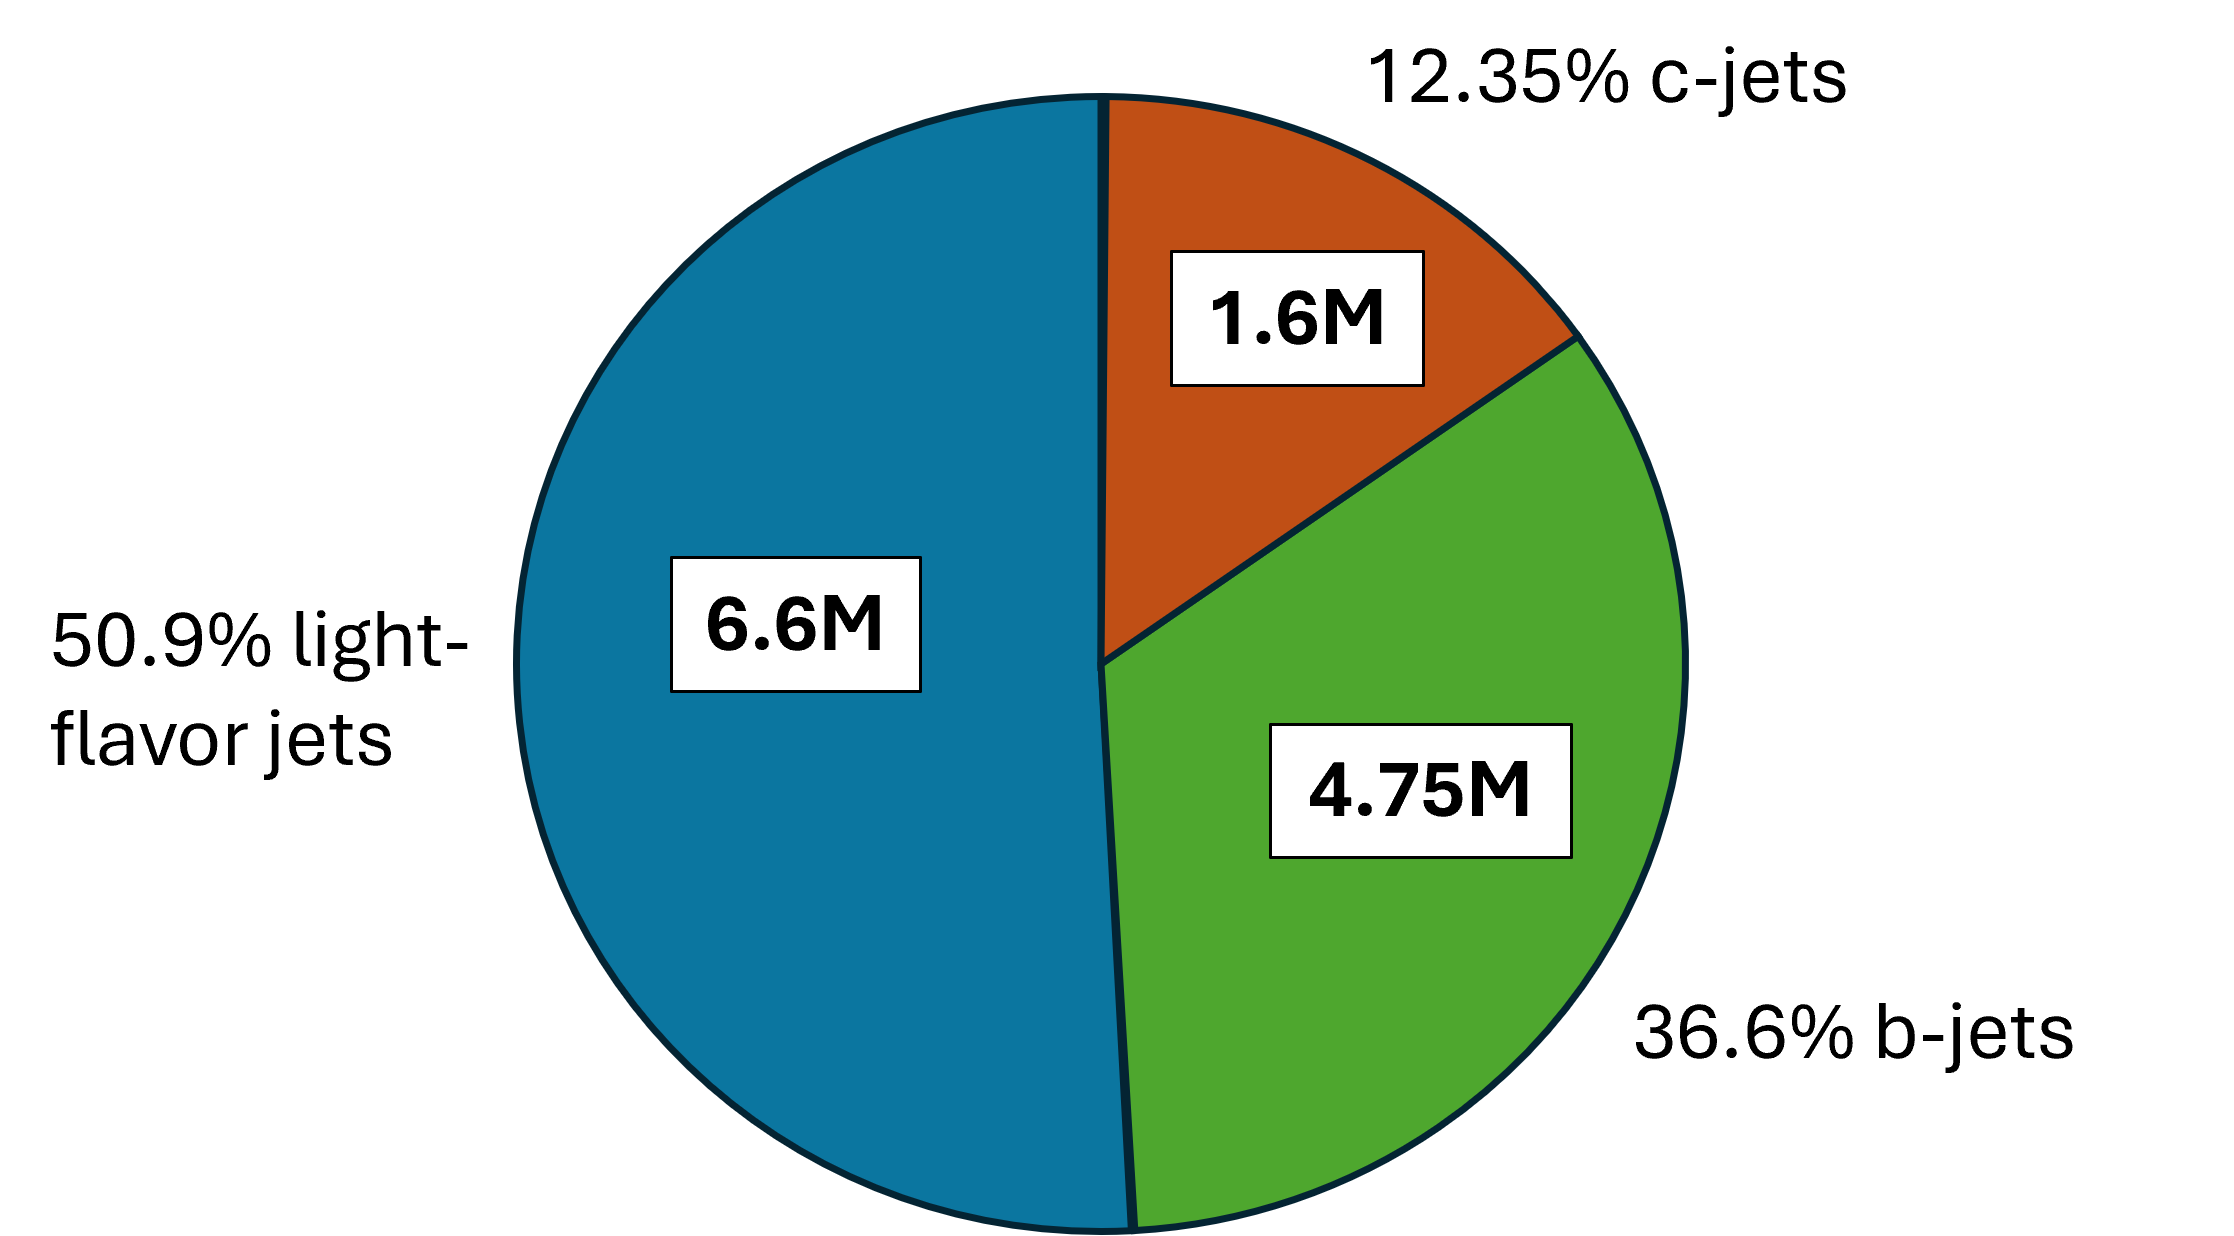
\includegraphics[scale=0.4]{figs/ch5/comp_pie.png}
    \caption{ Diagram of hadron composition in the HL-LHC MC samples.}
\label{fig:comp-pie}
\end{figure}

\hspace{-3mm}
\begin{table}[H]
    \centering 
    \begin{tabular}{ |c | c | c| c|}
        \hline
        \multicolumn{4}{|c |}{Dataset Compositions and Statistics}\\
        \hline\hline
        Dataset & Total Types of Jets & From: $t\bar{t}$ & From: $\textrm{Z}'$  \\
        \hline
        Training set & 4.75M b-jets & 4.1M & 650K \\
                     & 1.6M c-jets  & 900K & 700K \\
                     & 6.6M light-jets & 5.1M & 1.1M \\
        Validation set &    &  2.6M & 1.1M \\
        Testing sets   &    & 2.6M  & 1.1M  \\
        \hline
        \hline
        \multicolumn{2}{|c|}{PDF Resampling Method} & \multicolumn{2}{|c|}{Count Resampling Method} \\
        \hline
        \multicolumn{2}{|c|}{15M Training Jets} & \multicolumn{2}{|c|}{4.8M Training Jets} \\
        \hline
    \end{tabular}
    \caption{Dataset statistics used for training DL1d for the HL-LHC}
    \label{tab:training-stats}
\end{table}

\subsection{Training DL1d}

The training of the DL1d tagger for the \gls{hllhc} is only preliminary where the final version will have more of a dedicated optimization and increased statistics. The \gls{dips} tagger that is 
used as input for this preliminary version of DL1d for Upgrade was trained by a fellow graduate student and was trained using two electron selections. Within \gls{atlas}, four fixed values
of the electron discriminant are defined (similar to the \gls{wp} defined for b-tagging).
These \gls{wp}s for the electron selection cuts are referred to as \textit{VeryLoose}, \textit{Loose}, \textit{Medium}, \textit{Tight} cuts. These cuts are set by the efficiencies for 
identifying a prompt electron with $\textrm{E}_{\textrm{T}}$ = 40 GeV are 93\%, 88\%, 80\% for \textit{Loose}, \textit{Medium}, \textit{Tight} respectively \cite{ele-cut}. One \gls{dips} model contains a tighter 
\gls{wp} selection cut, and the other a loose \gls{wp} selection cut.  Therefore, four DL1d models are trained in total, two models trained using both of these cuts and 
being resampled via the count method and the other two using the PDF method. The DL1d architecture follows the deep feed-forward architecture shown in Figure \ref{fig:dl1-arch} but with specified nodes.
A diagram showing the specified node architecture can be seen in Figure \ref{fig:dl1d-arch}.

\begin{figure}[h]
    \centering
    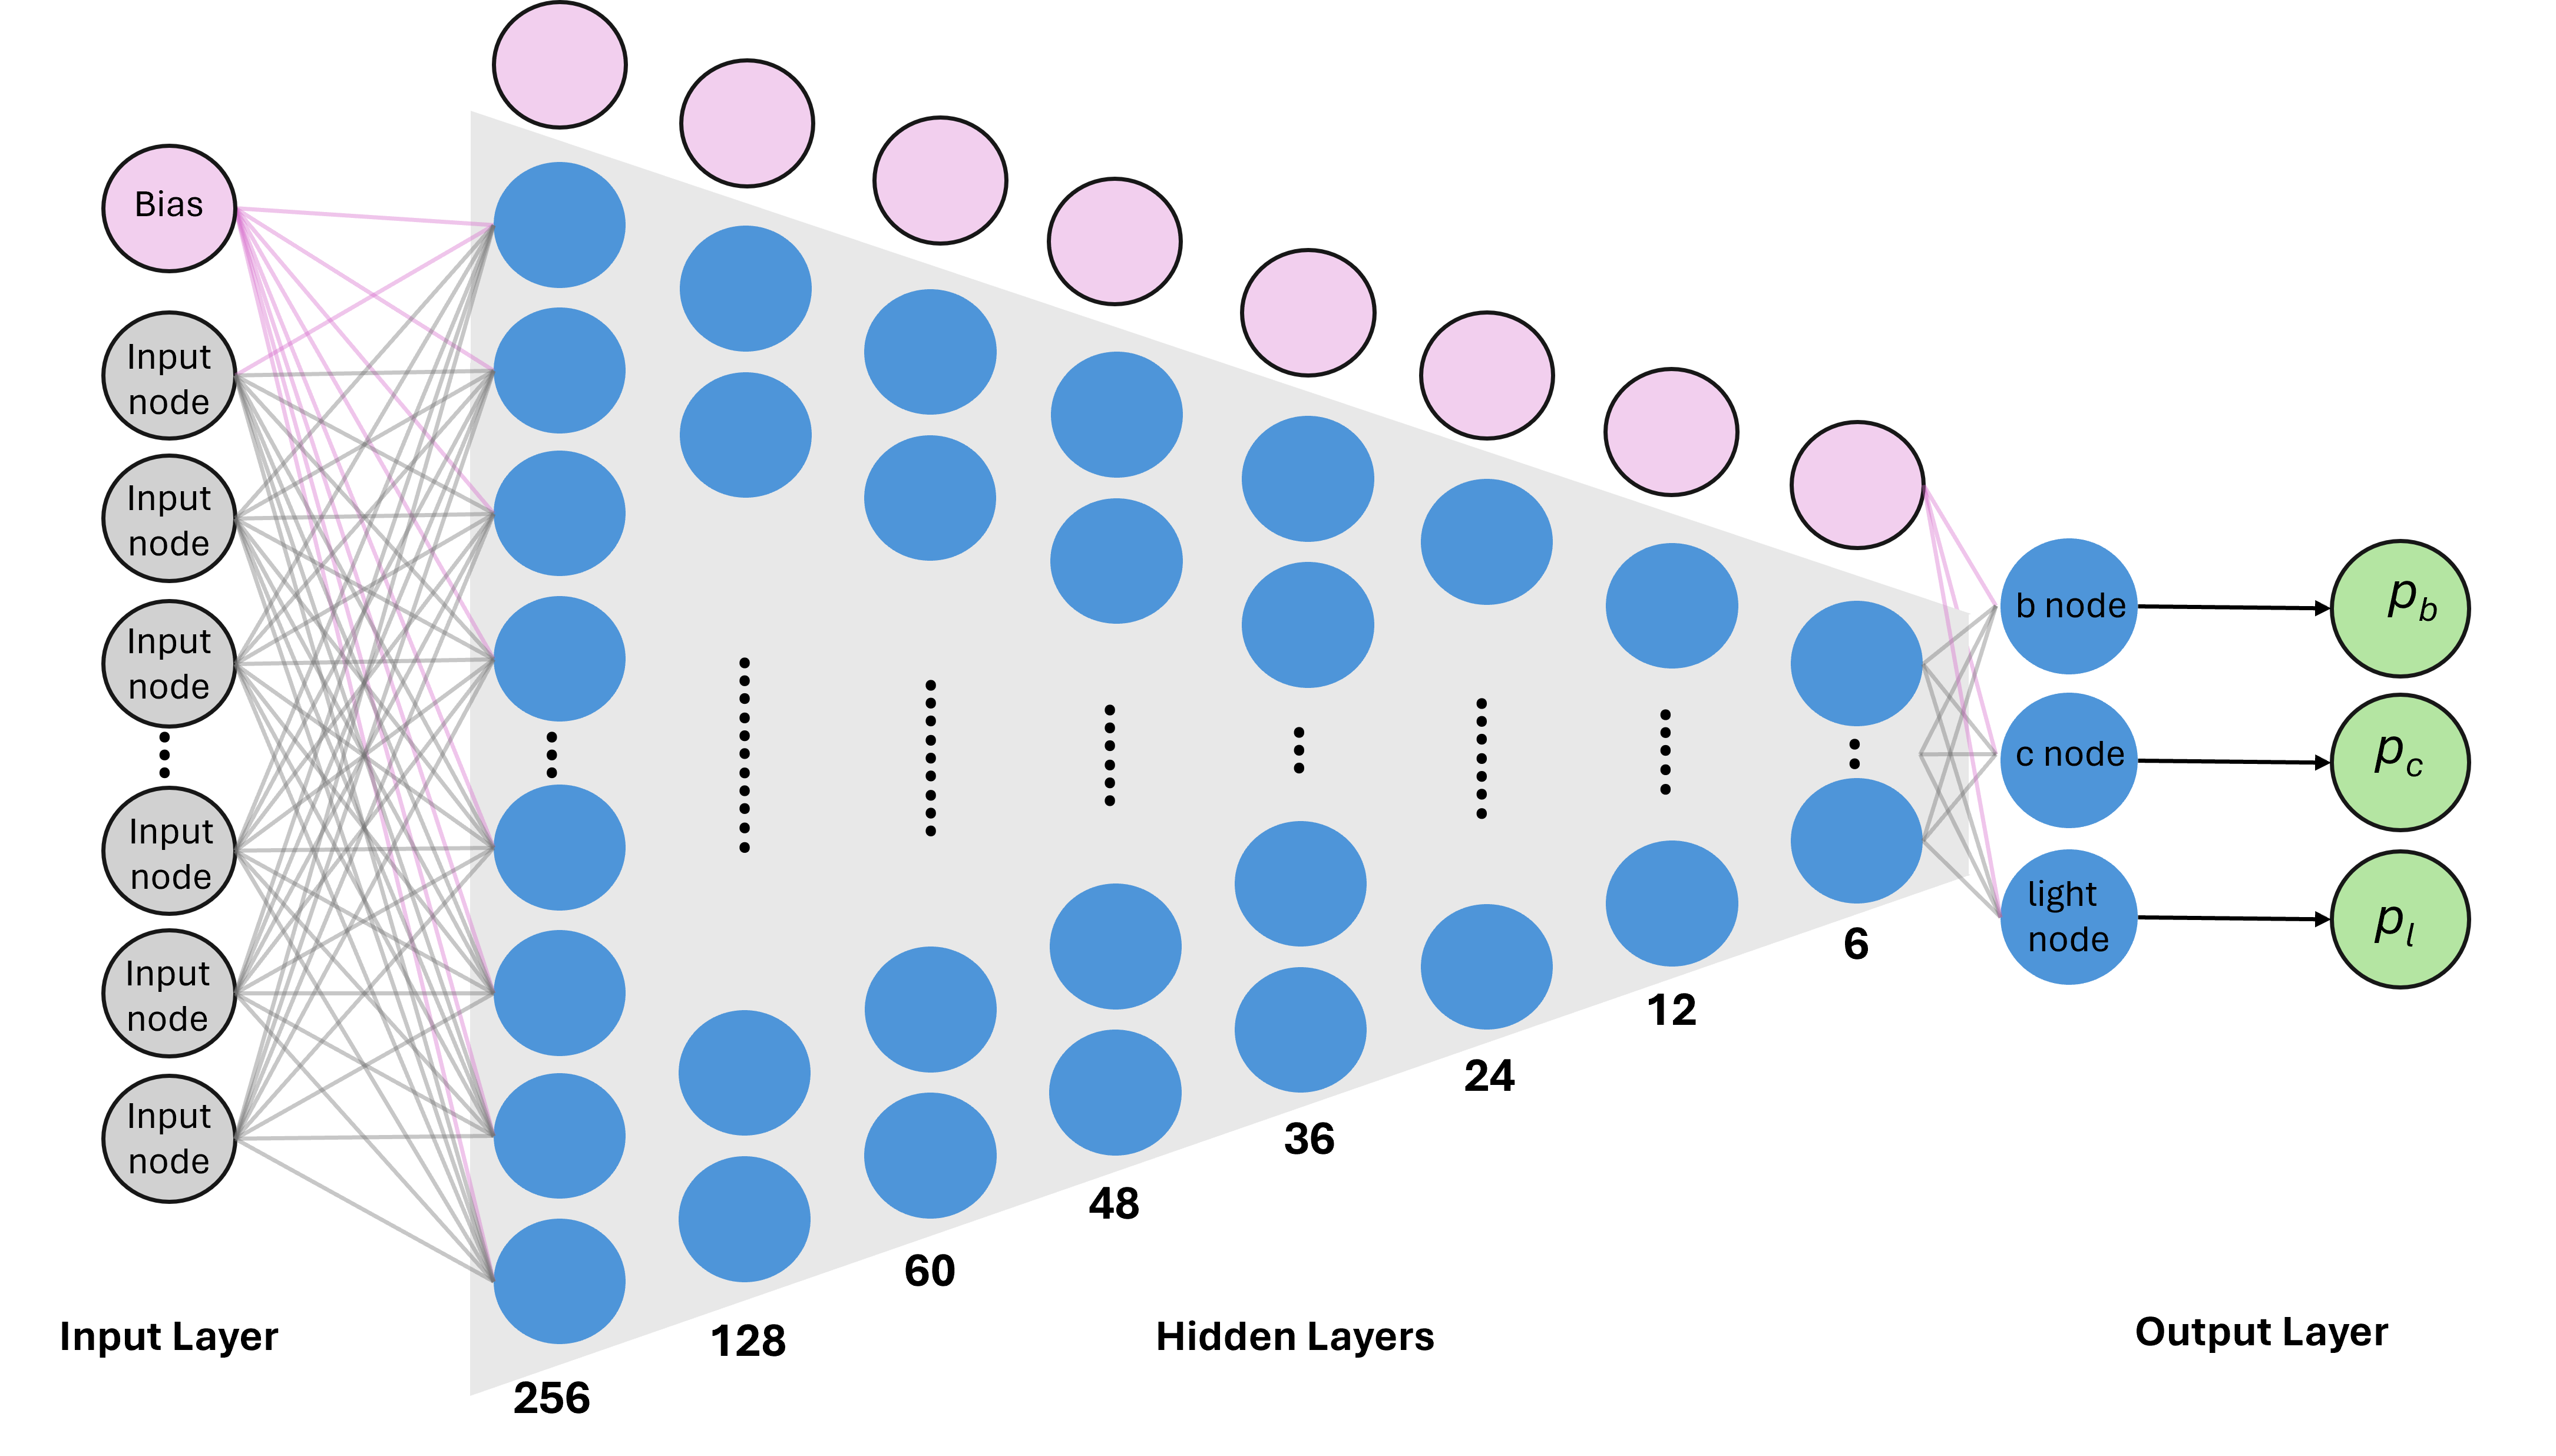
\includegraphics[scale=0.5]{figs/ch5/dl1d-arch.png}
    \caption{ Deep feed-forward architecture used for preliminary Upgrade DL1d model.}
\label{fig:dl1d-arch}
\end{figure}

Using the loss function described in Eq. \ref{eq:5.4}, the loss value is recorded per training epoch and plotted in Figure \ref{fig:vepoch} while 
also showing the loss of the associated \gls{dips} model used in the DL1d architecture. The loss is shown for the $t\bar{t}$ sample,
$\textrm{Z}'$ sample and the combined hybrid sample. Since the training is done on the hybrid sample, the loss function converges 
much quicker than just on the single samples. Figures \ref{fig:vepocha} and Figure \ref{fig:vepochb} shows the loss per epoch for both the PDF method and Count method, revealing 
that loss convergence stabilizes faster in the PDF method than the count. This is due to the increase of statistics, letting the model 
training being able to reliably find underlying patterns at a faster rate. Figures \ref{fig:vepochc} and \ref{fig:vepochd} shows the light-jet rejection rate with 
respect to the training epoch. This reveals the increase of effectiveness between the \gls{dips} model and the DL1d. Adding jet 
kinematic information from the baseline taggers to the underlying track structures from \gls{dips} massively increases light-jet 
rejection rate. Using the PDF resampling increases this rejection rate as seen between plots (c) and (d) in Figure \ref{fig:vepoch}. The convergence 
in the undersampling method Count takes about 100 more epochs, substantiating that the PDF resampling method is the superior approach. All 
these figures used the 77\% \gls{wp} for b-tagging. 


\begin{figure}[H]
    \centering
    \begin{subfigure}{0.45\textwidth}
        \centering
        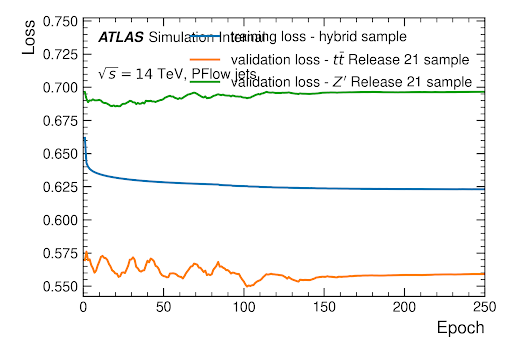
\includegraphics[width=\textwidth]{figs/ch5/lossvepoch_pdf.png}
        \caption{Loss per training epoch using PDF}
        \label{fig:vepocha}
    \end{subfigure}
    \begin{subfigure}{0.45\textwidth}
        \centering
        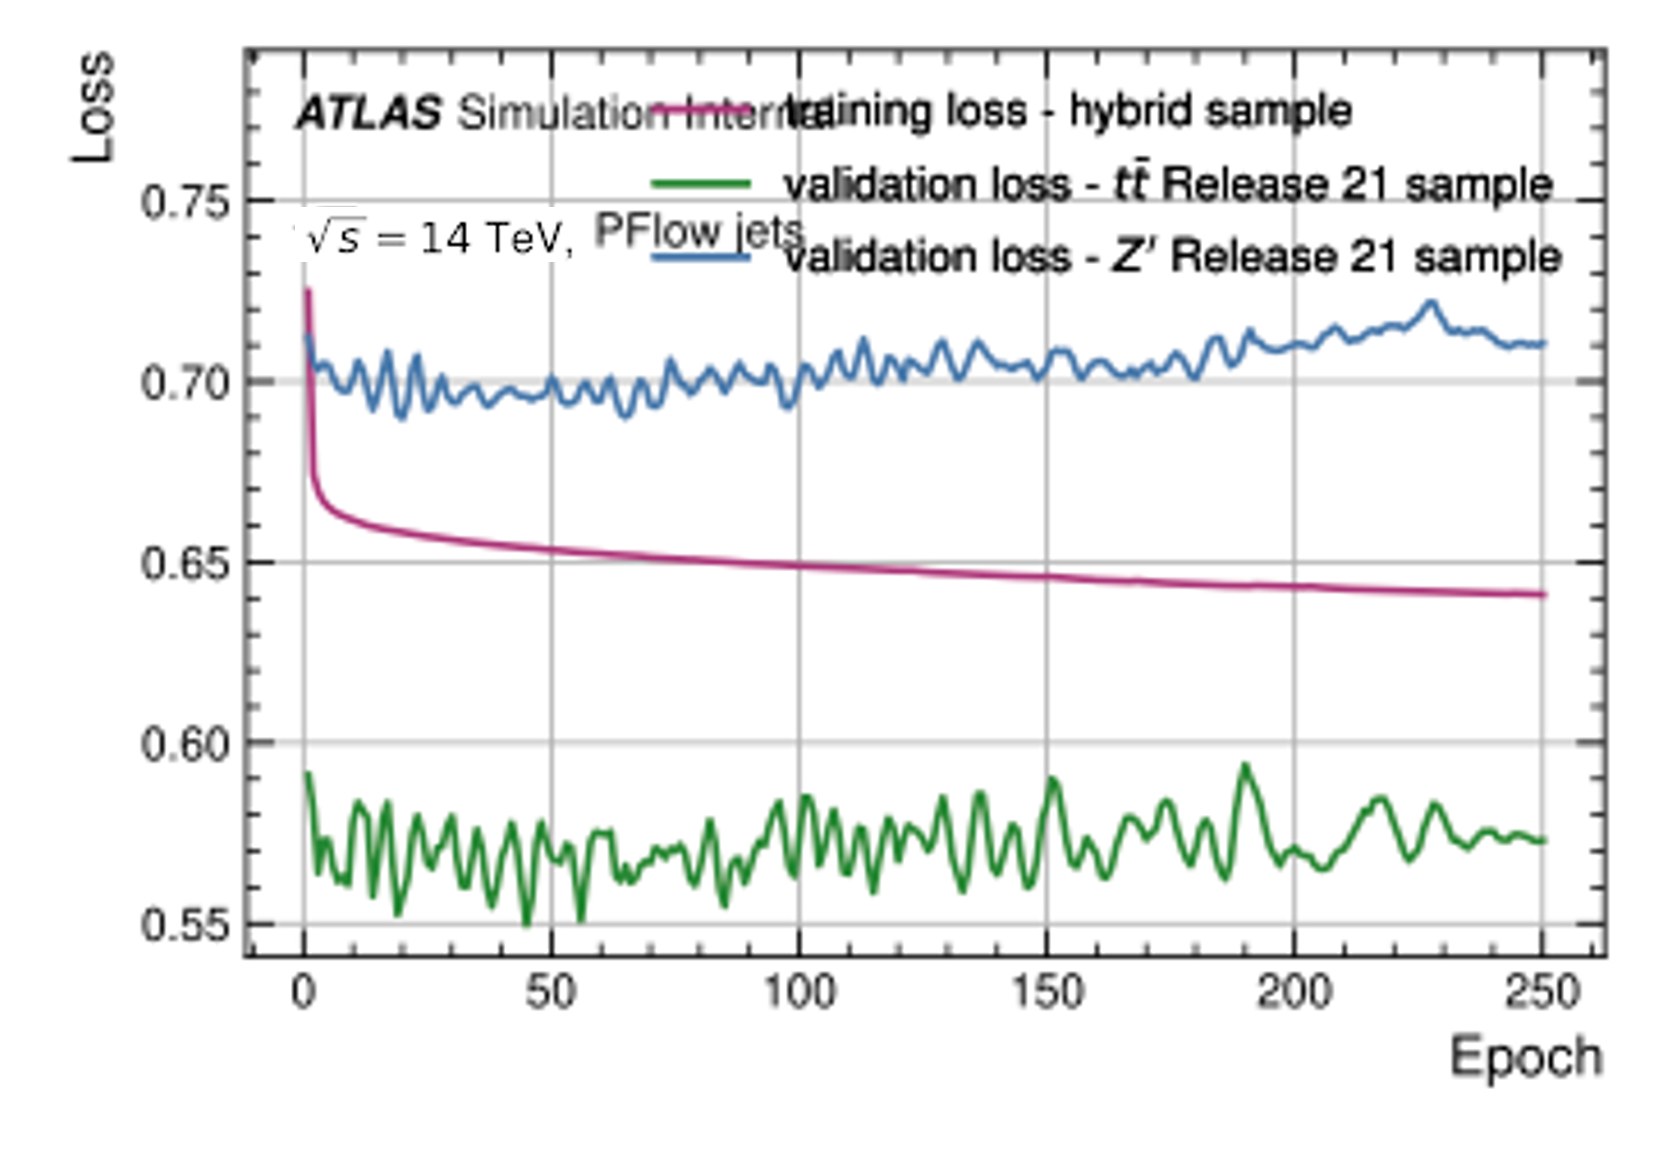
\includegraphics[width=\textwidth]{figs/ch5/lossvepoch_count.png}
        \caption{Loss per training epoch using Count}
        \label{fig:vepochb}
    \end{subfigure}
    \begin{subfigure}{0.45\textwidth}
        \centering
        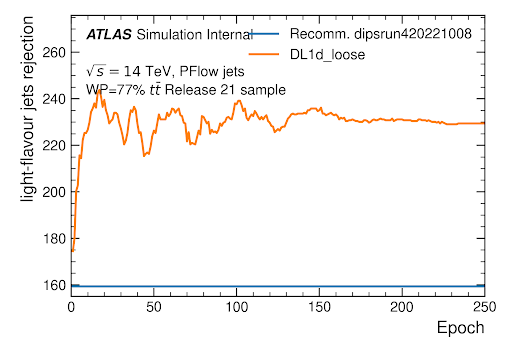
\includegraphics[width=\textwidth]{figs/ch5/rejvepoch_pdf.png}
        \caption{PDF light-jet rejection rate per epoch}
        \label{fig:vepochc}
    \end{subfigure}
    \begin{subfigure}{0.45\textwidth}
        \centering
        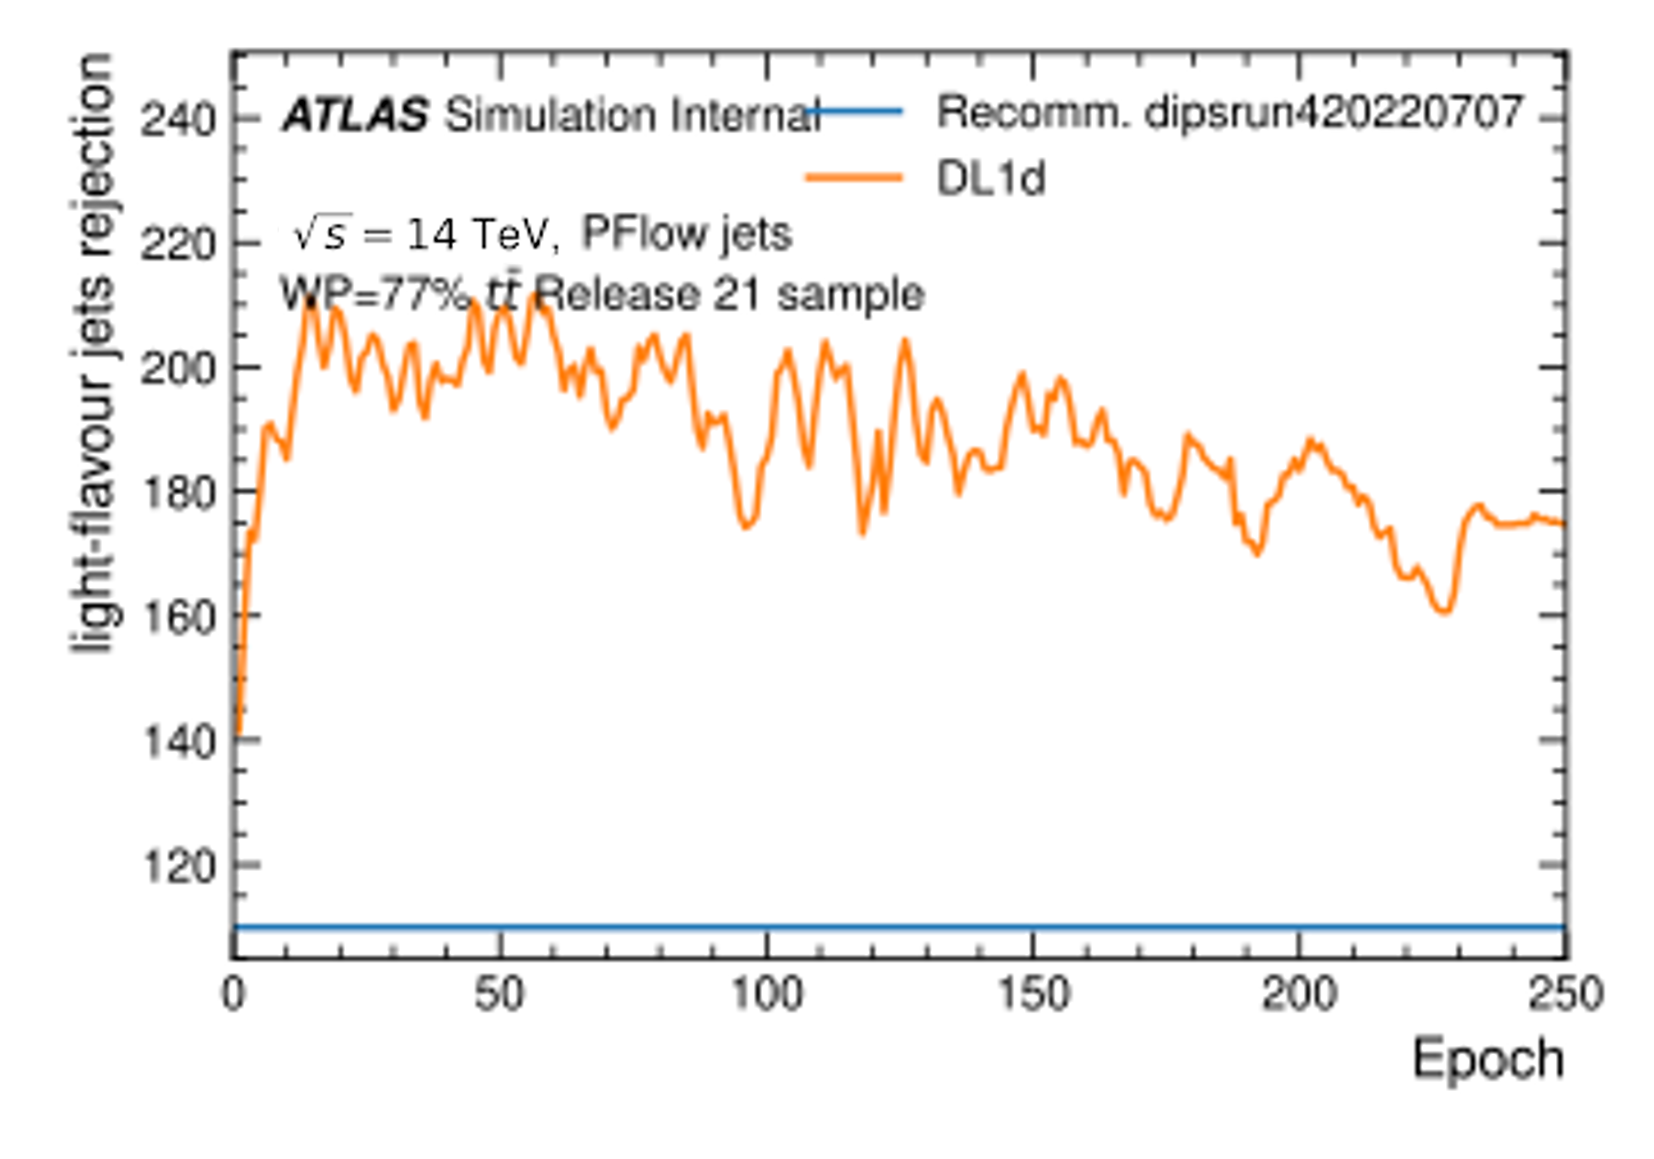
\includegraphics[width=\textwidth]{figs/ch5/rejvepoch_count.png}
        \caption{Count light-jet rejection rate per epoch}
        \label{fig:vepochd}
    \end{subfigure}
    \caption{(a) Shows loss per training epoch using the PDF method for both DL1d and its associated DIPS model using the loose electron selection cut. 
    (b) Shows loss per training epoch using the count resampling method for both DL1d and its associated DIPS model using the loose electron selection cut.
    (c) Shows the light-jet rejection rate per training epoch using the PDF method. DL1d shows rejection at a higher efficiency. 
    (d) Shows the light-jet rejection rate per training epoch using the Count resampling method. DL1d outperform DIPS but does not has a lower rejection rate than using the PDF resampling method as seen in (c)}
    \label{fig:vepoch}
\end{figure}


In order to calculate the final discriminant scores, a fraction scan is implemented 
to find an effective c-jet fraction value for the float $\textrm{f}_{\textrm{c}}$ shown in Eq. \ref{eq:5.2}. Since light-jet rejection 
and c-jet rejection are both affected by the chosen floating value, it's optimized to have a balanced effect in the $t\bar{t}$ sample while 
favoring c-jet rejection in the $\textrm{Z}'$ sample. The fractions are taken at the 77\% \gls{wp}. The scan can be seen in Figure \ref{fig:cfrac}.
Table \ref{tab:c-perc} shows the actual percentage value of c-hadrons within each sample. The value of 9\% was chosen for $\textrm{f}_{\textrm{c}}$ 
and can be seen in Figure \ref{fig:cfrac} at the point marked by the red \textit{X}. 


\begin{table}[H]
    \centering 
    \begin{tabular}{ |c | c |}
        \hline
        \multicolumn{2}{|c |}{C Hadron Percentage}\\
        \hline\hline
        Dataset & percentage  \\
        \hline
        $t\bar{t}$ & 7\% \\
        $\textrm{Z}'$ & 9\% \\
        \hline
    \end{tabular}
    \caption{C-hadron percentages in both training samples prior to combining}
    \label{tab:c-perc}
\end{table}


\begin{figure}[h]
    \centering
    \subfloat[\centering ]{{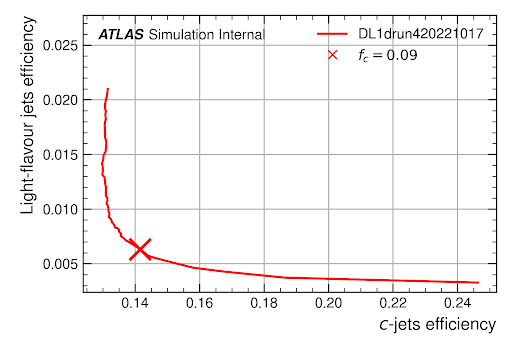
\includegraphics[scale=0.35]{figs/ch5/cfrac_ttbar.png}}}%
    \qquad
    \subfloat[\centering ]{{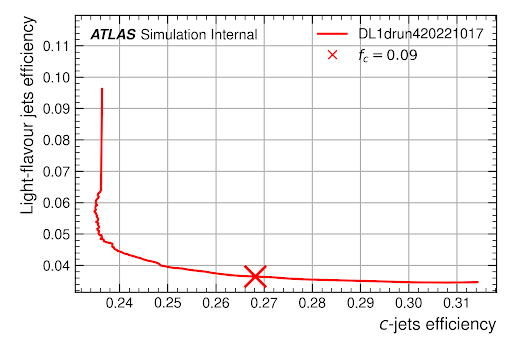
\includegraphics[scale=0.35]{figs/ch5/cfrac_zp.png}}}%
    \caption{ C-jet fraction scans for the float value $\textrm{f}_{\textrm{c}}$. The balancing value chosen is marked by \textit{X} on both plots.
    The chosen value is 0.09, balancing the light-jet rejection and c-jet rejection in the $t\bar{t}$ sample while favoring c-jet rejection in the $\textrm{Z}'$ sample.}
\label{fig:cfrac}
\end{figure}

Since four models were trained using both resampling methods (PDF and Count) while using two different \gls{dips} models that use different electron cuts, they had to be compared to see which 
model outperforms the other three. While holding the optimized value of $\textrm{f}_{\textrm{c}}$ = 0.09, the b-jet tagging efficiency was checked for all the models. Figure \ref{fig:dl1d-comp} shows a Receiver Operating Characteristic (\gls{roc}) curve. This shows background rejection vs b-tagging efficiency. The goal for these models is to have the highest rate of b-tagging efficiency while 
rejecting the most amount of background. The bottom two plots below the \gls{roc} curve are two ratio plots showing the efficiency of the DL1d models with respect to the DL1d using the Count 
resampling method. The left plot validates the models on the $t\bar{t}$ sample while the right validates them on the $\textrm{Z}'$ sample. It's quite noticable on the $t\bar{t}$ sample plot that 
using the loose electron cut dramatically increases the DL1d performance b-tagging efficiency. As seen in pink on the right plots in Figure \ref{fig:dl1d-comp}, the model DL1d + the loose electron cut \gls{dips} 
model outperforms the other three while being comparable in the $t\bar{t}$ plot on the left. Therefore, the DL1d model with the loose electron selection cut was taken as the best model and was used 
in the following comparison plots for the rest of this section.

\begin{figure}[h]
    \centering
    \subfloat[\centering ]{{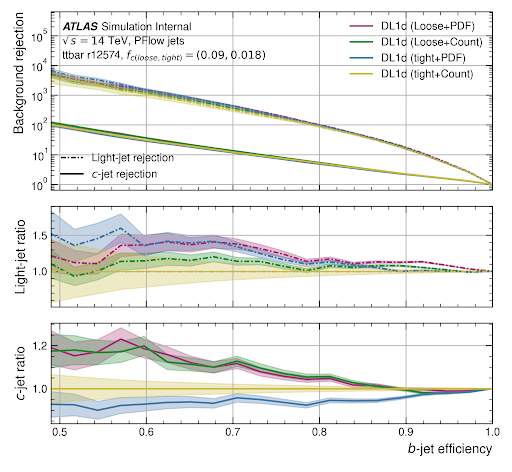
\includegraphics[scale=0.43]{figs/ch5/rejveff_ttbar.png}}}%
    \qquad
    \subfloat[\centering ]{{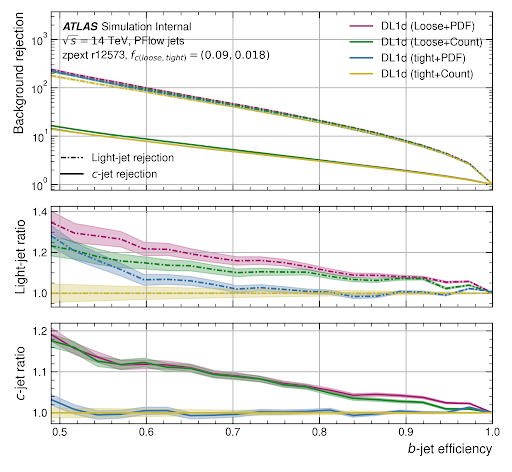
\includegraphics[scale=0.43]{figs/ch5/rejveff_zp.png}}}%
    \caption{ Comparison plots of all four DL1d trained models. Plot (a) shows the performance of each model using the $t\bar{t}$ sample. Both loose electron WPs outperform the tight WP. Plot (b) shows
    all four DL1d models validated on the $\textrm{Z}'$ sample. Again, both loose electron WPs models outperform the tight WPs while the PDF resampling method (pink) outperforms the Count method (green).
    The loose DL1d model using the PDF resampling method was chosen to be the superior trained model. }
\label{fig:dl1d-comp}
\end{figure}

Once the optimum model was chosen, the next step was to check on how the performance of it compares to the baseline \gls{dips} model. It is expected for the DL1d model to greatly outperform 
the \gls{dips} model simply due to the fact that the jet kinematics are added after the training of \gls{dips}, increasing the underlying pattern recognition from the excess of available information. 
This performance can be seen in Figure \ref{fig:dl1d-dips-comp}. As expected, the DL1d model outperforms the baseline \gls{dips} model by approximately 25\% in c-jet rejection vs b-tagging efficiency.

\begin{figure}[h]
    \centering
    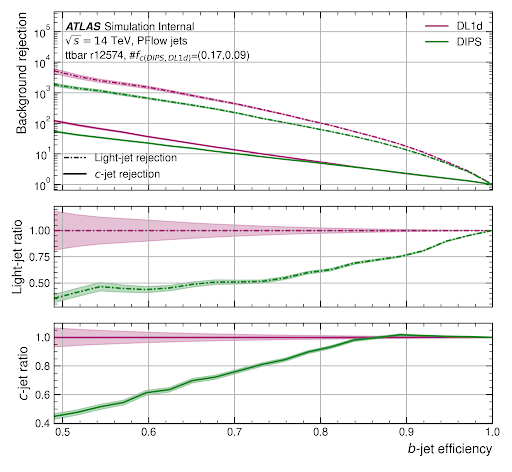
\includegraphics[scale=0.75]{figs/ch5/rejveff_dl1dcdips.png}
    \caption{ Comparison plot for the DL1d model and the baseline DIPS. DL1d outperform DIPS as expected. The c-jet fraction for the DIPS model was taken to be $\textrm{f}_{\textrm{c}}$ = 0.17 whereas 
    this fraction was $\textrm{f}_{\textrm{c}}$ = 0.09 as previously stated. }
\label{fig:dl1d-dips-comp}
\end{figure}

Just as in testing the model's b-tagging efficiency, the c-tagging efficiency can also be checked using the discriminant seen in Eq. \ref{eq:5.2}. The following plots show the performance of both 
the DL1d and the baseline \gls{dips} tagger for c-tagging efficiency. The DL1d tagger outperforms the \gls{dips} as expected just as in the b-tagging study. For these plots, the \gls{hgtd} sample 
was used as listed in Table \ref{tab:dl1-samples}. Two performances are shown for two different floating b-jet fractions $\textrm{f}_{\textrm{b}}$ as seen in Eq. \ref{eq:5.2}. The left plot 
has a floating b-jet value of $\textrm{f}_{\textrm{b}}$=0.24 and the right plot has a value of $\textrm{f}_{\textrm{b}}$=0.45.

\begin{figure}[h]
    \centering
    \subfloat[\centering ]{{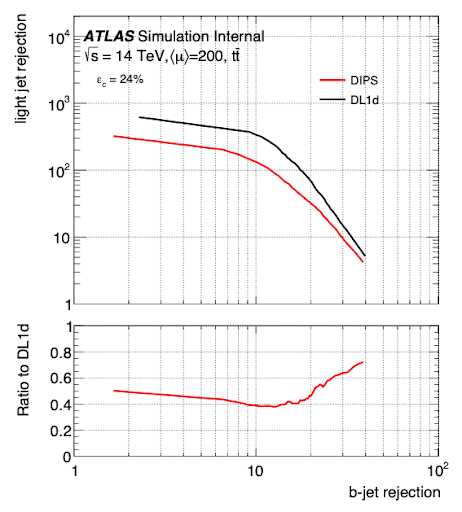
\includegraphics[scale=0.45]{figs/ch5/brej24c.png}}}%
    \qquad
    \subfloat[\centering ]{{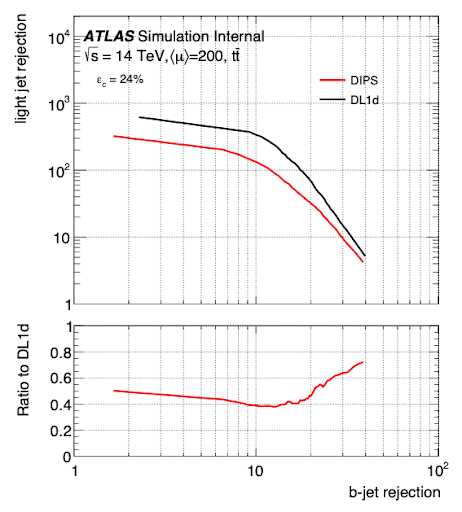
\includegraphics[scale=0.45]{figs/ch5/brej45c.png}}}%
    \caption{ Light-jet rejection vs b-jet rejection (c-tagging). The left plot has a floating fraction of $\textrm{f}_{\textrm{b}}$=0.24 where as the right has $\textrm{f}_{\textrm{b}}$=0.45. The DL1d
    tagger outperforms DIPS as expected. The small HGTD sampled as listed in Table \ref{tab:dl1-samples} was used. }
\label{fig:dl1d-ctag}
\end{figure}

This DL1d tagger was the first of its kind to be trained on samples with the geometry of \gls{atlas} in Run 4. With the increase of luminosity within the \gls{hllhc} and the upgrades in timing 
resolution and granularity within the \gls{itk} and \gls{hgtd}, tagging efficiencies is expected to increase. It has proved to be difficult to train a preliminary tagger to outperform the current 
state-of-the-art taggers. Though, at the current state, this is to be expected for several reasons. One would expect the tagging efficiency to increase with the amount of available statistics to train on.
This preliminary DL1d using Upgrade samples had a total of $\approx$15 million jets to train on that include jets between the newly included eta range of 2.4 $<|\textrm{η}|<$ 4.0 (total range of 0 $<|\textrm{η}|<$ 4.0) 
which may not include well resolved jets. The current state-of-the-art DL1d tagger was trained using 120 million jets simulated using Run 2 \gls{atlas} geometry with well resolved jets between the 
eta range of  0 $<|\textrm{η}|<$ 2.4. The comparison of these two versions of DL1d can be seen in Figure \ref{fig:dl1d-mv2-comp}. This figure also includes the old high-level tagger of \gls{mv2} that was validated on 
samples with the inclusive eta range of 0 $<|\textrm{η}|<$ 4.0. In this comparison \gls{roc} plot, it is seen that the DL1d for Run 2 outperforms the preliminary DL1d for Upgrade up to the 77\% \gls{wp} but starts to under perform at the 85\% \gls{wp} in the light-jet rejection. This result is highly promising knowing the robustness of the Run 2 version. If a more refined DL1d for Upgrade model is trained using 
an increase in statistics, it would be expected to outperform the Run 2 DL1d at the 77\% \gls{wp}.

\begin{figure}[h]
    \centering
    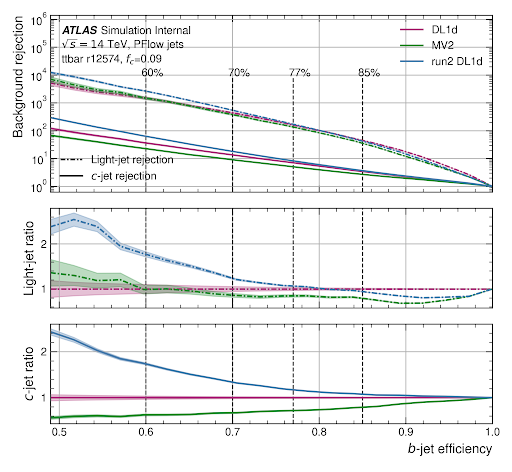
\includegraphics[scale=0.75]{figs/ch5/rejveff_mv2.png}
    \caption{ ROC curve comparing the performance of the DL1d for Run 4, the current version of DL1d used for Run 2 and the MV2 high-level tagger.}
\label{fig:dl1d-mv2-comp}
\end{figure}

Adding the newly available eta region of 2.4 $<|\textrm{η}|<$ 4.0 through the calculated power of the \gls{itk} detector has physicists excited about the new 
aspects that this adds to their analyses and possible innovations in the future. Though, in order to effectively probe this region, the available \gls{ftag}
high-level taggers must be trained with robustness. Due to the decreasing resolution as particles become highly boosted in a more forward region of the detector,
it is expected for particle tagging efficiency to drop. Thus, requiring newer innovative tools and techniques to be implemented with the hopes to obtain the maximum efficacy of this new phase space. The high-level tagger DL1d has been state-of-the-art through the end of Run 2 and into Run 3 of the \gls{atlas} detector's 
campaign lifetimes. The question is how well will this tagger perform during Run 4 within the extended eta region. Figure \ref{fig:dl1d-eta-comp} shows its current performance 
in increasing eta intervals of one. The performance in the highly boosted region between 3 $<|\textrm{η}|<$ 4.0 shows the poorest performance but this is 
to be expected. The Upgrade DL1d model was also validated on jets that are only contained in the eta region 0 $<|\textrm{η}|<$ 2.5 to have a proper comparison 
between the current implemented Run 2 DL1d tagger. The ratio plot on Figure \ref{fig:dl1d-eta-comp} shows the performance between these two taggers. Similar performance is seen at 
the 77\% \gls{wp} with an increasing performance above this value. This result is very promising since the Run 4 version of the DL1d tagger was trained on a 
magnitude less of statistics.
\par
Overall, this first preliminary study of the high-level tagger DL1d using samples that simulate the Upgrade geometry of the \gls{atlas} detector during Run 4 
and the first implementation of the \gls{hllhc} shows very promising results.  
There are currently active efforts to develop a new state-of-the-art high-level tagger using a graph neural network on tracking information called \gls{gn1}. 
The architecture was briefly discussed in Section \ref{sec:gn1}. Preliminary studies of this new tagger were done using the same samples that 
were used in this study of Run 4 for DL1d. The results of this study are discussed in Appendix \ref{appendix:gn1-upgrade}. As seen from the results of this \gls{gn1} tagger,
it outperforms the DL1d tagger. Due to this, a graph neural based tagger is planned to be considered the new industry used tagger after the upgrade in 2029. Therefore, 
further studies of the DL1d tagger using larger Upgrade samples is not planned for and the model trained in this dissertation will be used at the DL1d baseline model for Upgrade. 

\newpage

\begin{figure}[H]
    \centering
    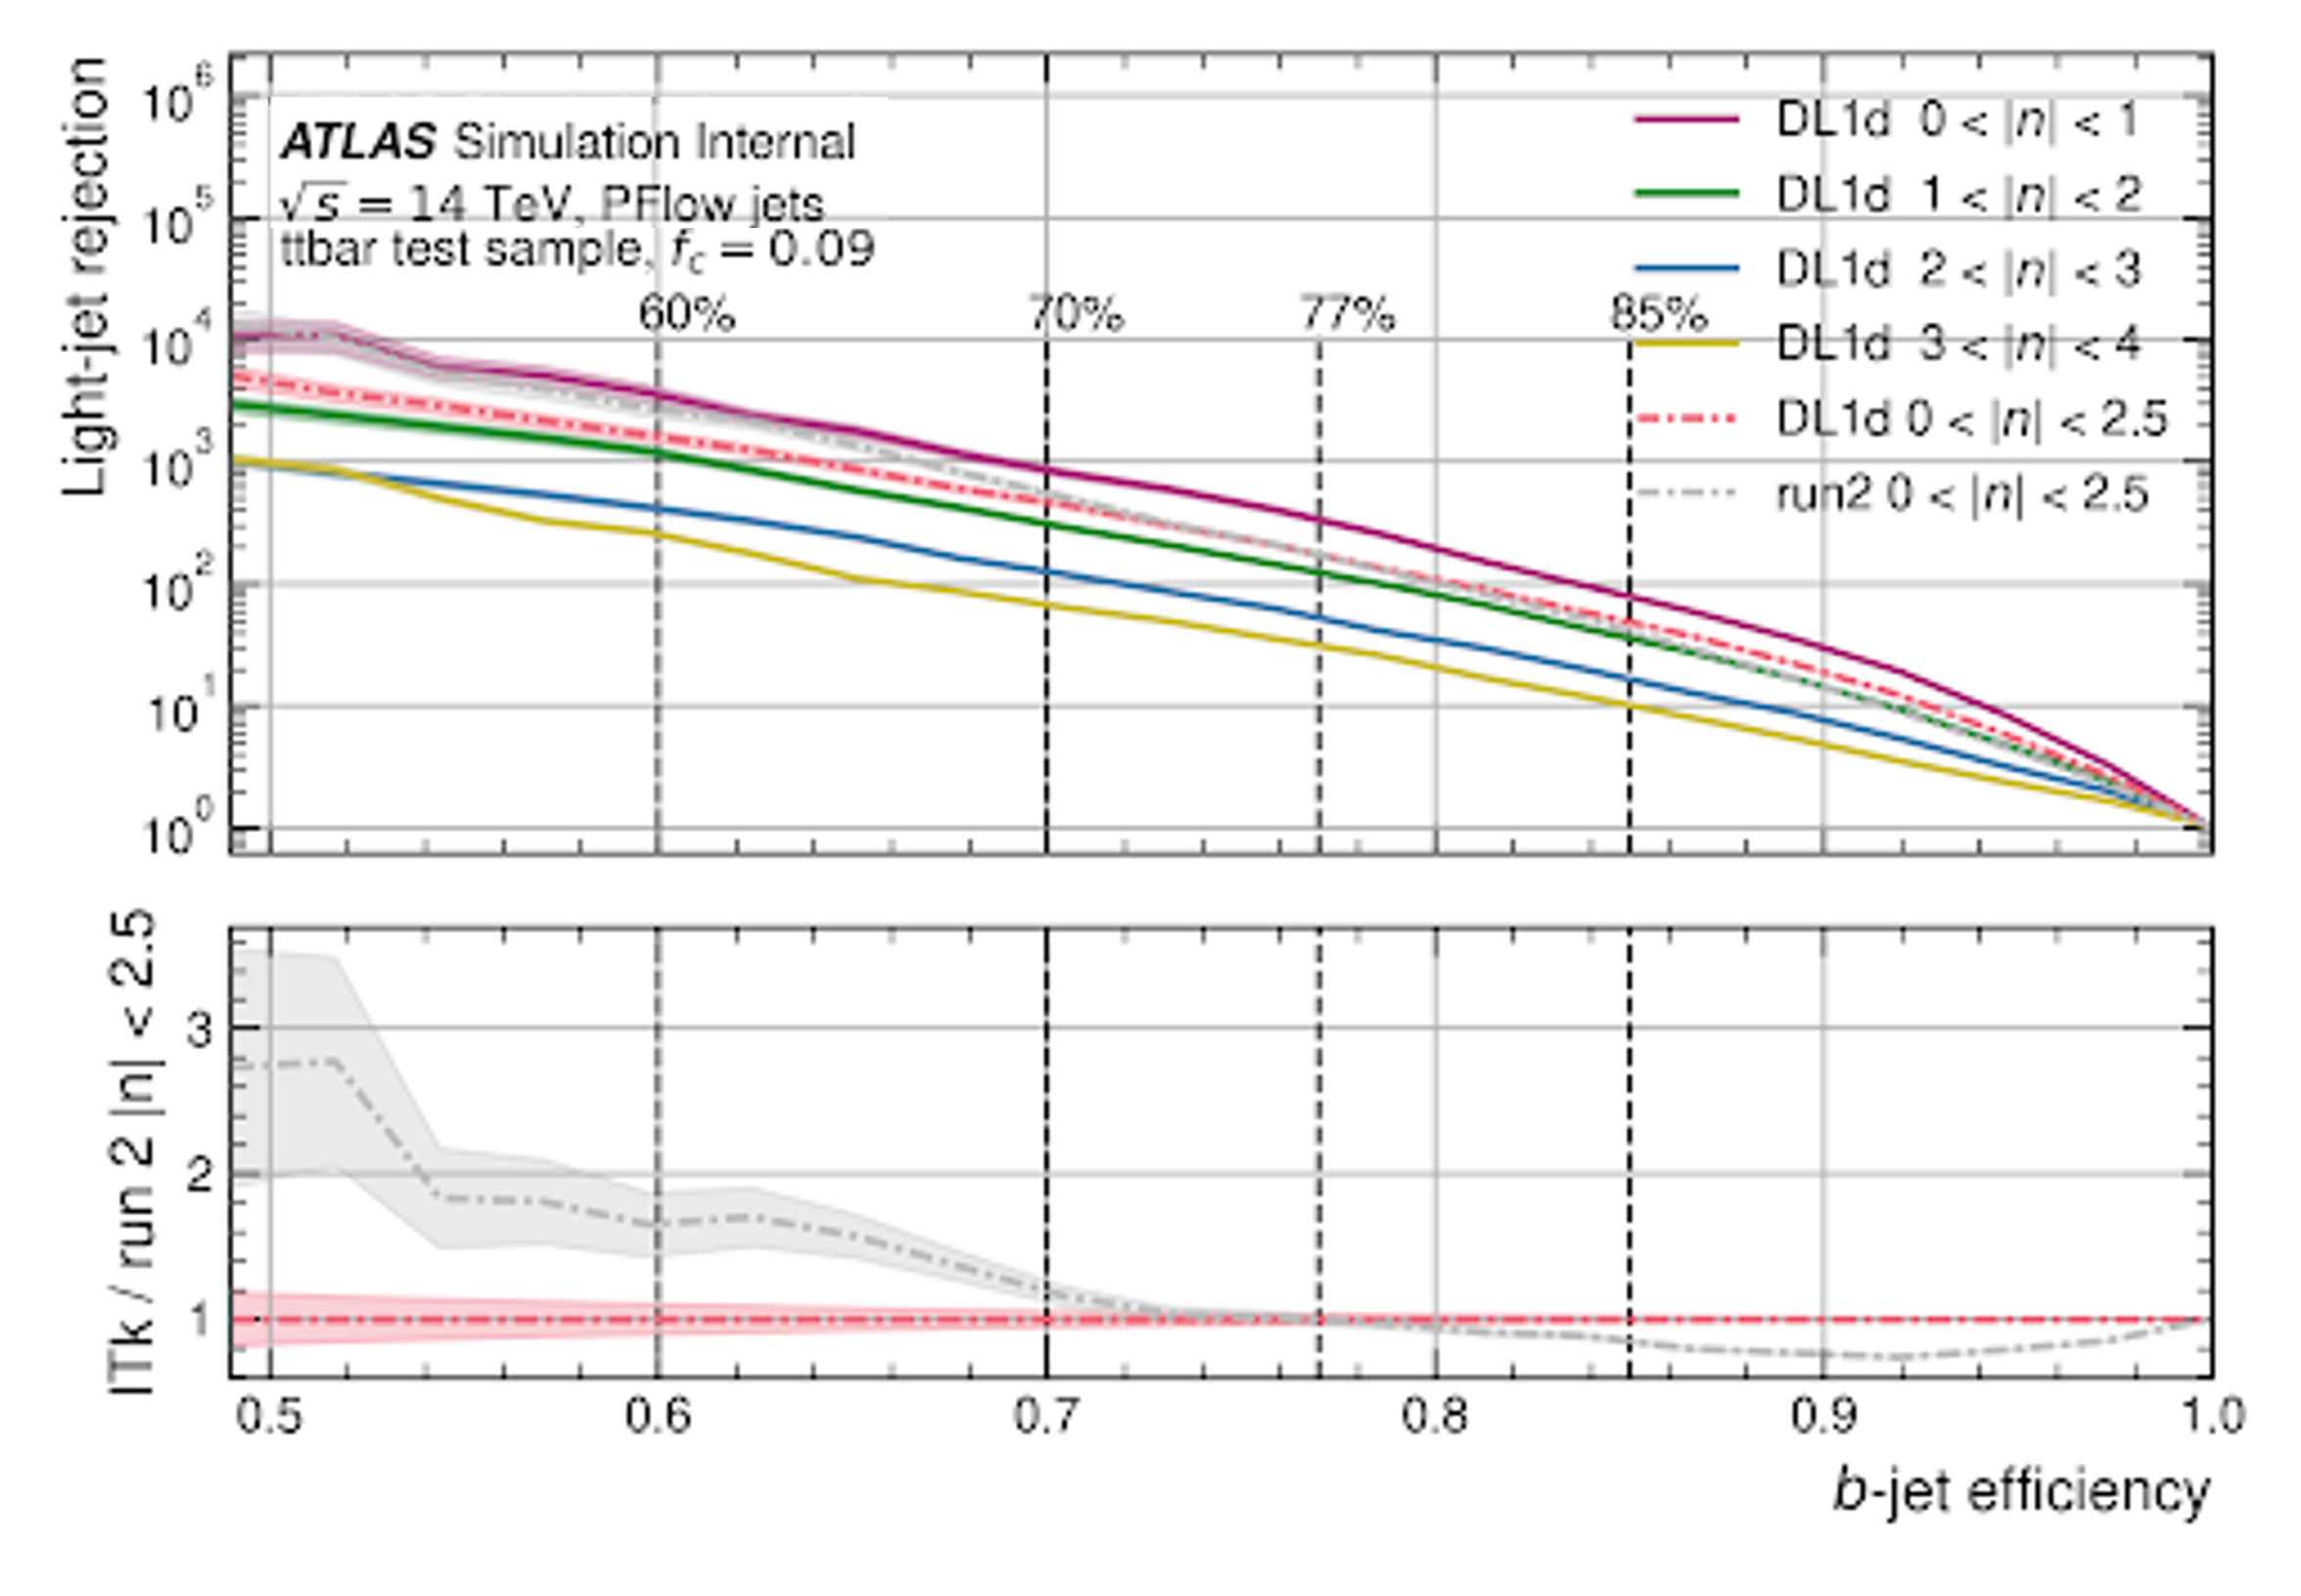
\includegraphics[scale=0.75]{figs/ch5/rejveff_eta.png}
    \caption{ ROC curve showing the performance of the DL1d tagger for Upgrade in four eta intervals of one. The Run 2 DL1d is also plotted for comparison in the ratio plot on the bottom.}
\label{fig:dl1d-eta-comp}
\end{figure}
